\documentclass[twoside,spanish,a4paper,12pt]{tfg}

% Editar la titulación
\titulacion{Grado en Ingeniería \\ Tele-Info-Multi}

% Editar el título
\title{Este es un muy largo título usado de prueba para ver cómo se formatea en varias líneas en la portada}

% Si es una alumna se debe usar
% \authorlabel{Autora}
\authorlabel{Autor}
% Editar el nombre
\author{Mi nombre}


% Si hay varios tutores:
% \tutorlabel{Tutores}
% \tutor{Nombre del tutor 1 \\[2mm] Nombre del turor2}
% Si el tutor es masculino:
% \tutorlabel{Tutor}
\tutorlabel{Tutora}
% Editar
\tutor{El nombre de la tutora}

% Editar: Poner mes y año de la convocatoria de lectura del TFM
\convocatoria{Julio 2020}

\begin{document}

% NO QUITAR ESTOS ELEMENTOS
\portada
\cleardoublepage
\contraportada
\cleardoublepage
\declaracion
\cleardoublepage


% Editar: Resumen en Español (obligatorio)
\begin{resumen}
  Este es el resumen del TFM. Debe ser corto (máximo media página) y cubrir los aspectos principales del TFM.
\end{resumen}
\cleardoublepage

% Editar: Resumen en Inglés
\begin{abstract}
  This is the abstract of the TFM. It must be short and cover the main aspects of the TFM.
\end{abstract}
\cleardoublepage

% Editar: Resumen en Valenciano
\begin{resum}
  Aquest és el resum del TFM. Ha de ser curt (màxim mitja pàgina) i cobrir els aspectes principals del TFM.
\end{resum}
\cleardoublepage


% Editar: Agradecimientos (opcional)
\begin{agradecimientos}
  En primer lugar quiero agradecer a todos aquellos que me han apoyado durante todos estos años.

  En segundo lugar...
\end{agradecimientos}
\cleardoublepage

\tableofcontents

\pagestyle{tfg}
\justify

% Las figuras se buscan en el directorio figs

% Cada capítulo está en su propio fichero tex. Ver el directorio tex.

% La bibliografía está dentro del directorio bib
\chapter{Introducción}
% Contenidos del capítulo.
% Las secciones presentadas son orientativas y no representan
% necesariamente la organización que debe tener este capítulo.

\section{Introducción}

La industria de los videojuegos ha sido testigo de una transformación excepcional en los últimos años. La búsqueda constante de experiencias más inmersivas y visualmente impresionantes ha llevado a los desarrolladores a explorar nuevas formas de crear mundos virtuales. En este contexto, la generación procedural de terrenos se ha convertido en una herramienta esencial para satisfacer las demandas de los jugadores cada vez más exigentes y hambrientos de autenticidad.

Este Trabajo de Fin de Máster (TFM) se adentra en el emocionante campo de la generación procedural de terrenos en Unity, uno de los motores de desarrollo de videojuegos más utilizados tanto por la industria como por desarrolladores independientes, pero con quiero continuar con esta introducción sin hacer una mención especial a Sebastian Lague, creador de contenido especializado en gráficos por computador cuyos tutoriales y proyecto sobre generación de terreno procedural sirvieron de base y de guía para la realziación de ste proyecto.

Siguiendo con el objetivo de este proyecto, este TFM tiene como meta diseñar y desarrollar una herramienta avanzada que permita a los creadores de juegos generar terrenos de manera eficiente y convincente.

Los datos disponibles, incluidos los proporcionados por fuentes como Eurostat y otros informes, indican un crecimiento constante en la industria de los videojuegos. A medida que la audiencia se expande, también lo hacen sus expectativas. Los jugadores contemporáneos buscan experiencias de juego que sean únicas y estimulantes. En este contexto, la generación procedural de terrenos se plantea como una solución que puede hacer posible la creación de mundos tanto auténticos como sorprendentes.

La historia de la generación procedural de terrenos comenzó con la implementación de algoritmos basados en ruido, entre los que destaca el renombrado Perlin Noise, desarrollado por Ken Perlin en la década de 1980. A pesar de que estos enfoques ofrecieron resultados impresionantes para su época, a menudo carecían de la autenticidad y el realismo que los jugadores modernos esperan en la actualidad. Con el aumento de la demanda de experiencias de juego más inmersivas y visualmente impactantes, se volvió crucial mejorar las técnicas de generación de terrenos.

Un avance destacado en este ámbito fue la introducción del Simplex Noise, una mejora significativa respecto al Perlin Noise, que mantuvo la capacidad de generar terrenos naturales, pero con un rendimiento más eficiente. No obstante, lo que realmente marcó un hito en la generación procedural de terrenos fue la incorporación de algoritmos de erosión. Estos algoritmos simulan procesos geológicos y climáticos, lo que resulta en terrenos con características naturales más convincentes, como montañas, cañones y ríos. Esta adición permitió crear mundos virtuales más realistas y creíbles, lo que contribuyó a elevar la calidad general de los juegos.

La creciente popularidad de los mundos abiertos en los videojuegos presentó un desafío significativo: generar terrenos continuos y sin interrupciones notables cuando los jugadores exploran los límites del mundo virtual. A medida que los algoritmos mejoraron, los juegos pudieron ofrecer experiencias de juego más fluidas y expansivas, lo que aumentó la inmersión del jugador y su sensación de exploración sin restricciones.

La influencia de la generación procedural de terrenos no se limita únicamente a la creación de paisajes virtuales. Ha dejado una huella indeleble en otros aspectos de la generación procedural en la industria de los videojuegos. Esto incluye la generación de ciudades completas en juegos de mundo abierto, la creación de misiones y contenido diverso que aumenta la rejugabilidad, así como la generación de personajes y criaturas que dan vida a los mundos virtuales. Además, ha influido en la generación de texturas y elementos artísticos, permitiendo un ahorro significativo de tiempo y recursos en el desarrollo de juegos y animaciones. La música y los efectos de sonido también se benefician de la generación procedural, adaptando la banda sonora y la atmósfera del juego en tiempo real para acompañar la acción.

En la última década, hemos sido testigos de un aumento significativo en la adopción de la generación procedural de terrenos en la industria de los videojuegos. Esto marca un cambio notable en la forma en que los desarrolladores abordan la creación de entornos virtuales. Esta adopción creciente se ha visto impulsada por varios factores clave, como la capacidad de generar mundos virtualmente infinitos sin incurrir en costos prohibitivos de almacenamiento. Además, proporciona una experiencia de juego única en cada partida, lo que aumenta la rejugabilidad y la longevidad de un título. Esta estrategia también es esencial en la creación de mundos abiertos sin pantallas de carga notables entre escenarios o biomas, lo que mejora la inmersión del jugador.

La evolución de la generación procedural de terrenos ha estado intrínsecamente ligada a la constante innovación en algoritmos y técnicas. En los últimos años, se han desarrollado y refinado una variedad de enfoques que van desde la generación basada en ruido, como el Perlin Noise y el Simplex Noise, hasta técnicas más avanzadas que incorporan algoritmos de erosión y simulaciones físicas para lograr terrenos aún más realistas.

Uno de los desafíos cruciales en la generación procedural de terrenos, especialmente en entornos de mundo abierto, es la gestión eficiente de los "chunks" de terreno, pequeñas porciones de terreno que se generan y almacenan en memoria para luego ser cargadas y descargadas dinámicamente mientras el jugador se mueve a través del mundo virtual. Este proceso es esencial para mantener un rendimiento óptimo y evitar la carga excesiva de recursos en la memoria del sistema. Además, es fundamental asegurarse de que la transición entre diferentes chunks sea fluida y sin discontinuidades notorias, lo que garantiza una experiencia de juego inmersiva. En el contexto de la generación procedural de terrenos, se ha consolidado una técnica comúnmente empleada denominada "sistema de streaming" de terrenos. Este enfoque se encarga de gestionar la carga y descarga de fragmentos o "chunks" de terreno de manera dinámica en función de diversos factores, como la proximidad del jugador, la dirección de su movimiento y su campo de visión. Uno de los principales objetivos de este sistema es garantizar una transición fluida entre chunks adyacentes, evitando discontinuidades notorias que puedan afectar negativamente a la cohesión y la inmersión en el mundo virtual.

Además, se emplean algoritmos de detección de colisiones y de visibilidad para determinar qué chunks deben ser cargados y renderizados según la posición actual de la cámara del jugador. Estos algoritmos son cruciales para optimizar el rendimiento del juego, ya que permiten reducir la carga en la unidad central de procesamiento (CPU) y la unidad de procesamiento gráfico (GPU). En consecuencia, solo se procesan y muestran los chunks que son relevantes y visibles desde la perspectiva del jugador en ese momento particular. Esta estrategia de optimización contribuye significativamente a lograr una experiencia de juego fluida y eficiente en términos de recursos.

En lo que respecta al movimiento de la cámara del jugador y su influencia en la generación del terreno, se implementan técnicas de "nivel de detalle" (LOD, por sus siglas en inglés) dinámico. Esta técnica se encarga de ajustar la resolución y el nivel de detalle del terreno en tiempo real en función de la distancia entre la cámara y el terreno circundante. Cuando la cámara se acerca a un chunk de terreno en particular, se aumenta el nivel de detalle, lo que implica mostrar texturas de mayor calidad y una geometría más detallada. Por otro lado, cuando la cámara se aleja, se reduce el nivel de detalle para conservar recursos de hardware y mantener un rendimiento óptimo.

En este contexto, el uso del Job System de Unity ha ganado relevancia. Permite la optimización de procesos intensivos en CPU, como la modificación de mallas de terreno, lo que resulta en una mejora significativa del rendimiento en juegos que implementan generación procedural de terrenos.

\section{Motivación}

El desarrollo de la herramienta de generación procedural de terrenos en Unity se enmarca en un contexto dinámico y desafiante, impulsado por diversas motivaciones que abordan necesidades y aspiraciones cruciales.

La industria de los videojuegos se encuentra en constante evolución, y la búsqueda incesante de experiencias más inmersivas y visualmente impactantes impulsa a los desarrolladores a explorar nuevas formas de crear mundos virtuales. La generación procedural de terrenos se erige como una respuesta a esta demanda creciente. Esta técnica no solo permite satisfacer las expectativas de los jugadores modernos en términos de autenticidad y sorpresa, sino que también agiliza el proceso de desarrollo de videojuegos al proporcionar herramientas eficientes para crear entornos expansivos y convincentes.

La gestión eficiente de chunks de terreno, la optimización del "Job System" de Unity y la elección de algoritmos adecuados son áreas que requieren innovación y soluciones creativas. Esta necesidad de abordar y superar desafíos técnicos en el campo de la generación procedural de terrenos motiva el desarrollo de esta herramienta. La oportunidad de enfrentar estos desafíos y crear una herramienta que marque la diferencia en la industria es una fuerza impulsora clave.

Este proyecto se enmarca en el contexto de una industria de videojuegos en constante cambio y una demanda creciente de experiencias inmersivas. La búsqueda de soluciones técnicas innovadoras y la aspiración de contribuir al crecimiento de la comunidad de desarrolladores son las motivaciones que guían este esfuerzo. La generación procedural de terrenos en Unity tiene el potencial de transformar la forma en que se crean mundos virtuales, y este proyecto se esfuerza por lograr precisamente eso.
\newpage


\chapter{Estado del arte}
\section{Introducción}

La generación automática de paisajes en el mundo de los videojuegos ha experimentado una evolución constante debido a la creciente demanda de experiencias de juego más envolventes y visuales impactantes. En este documento, exploramos esta técnica en detalle, con un enfoque particular en su implementación en el motor de desarrollo de videojuegos Unity.

La generación automática de paisajes se ha convertido en una herramienta esencial para los desarrolladores de videojuegos, ya que les permite diseñar mundos virtuales expansivos y auténticos que satisfacen las expectativas cada vez más altas de los jugadores. Este proyecto se centra en las técnicas, algoritmos y herramientas que han impulsado esta disciplina en la última década. A continuación, desglosaremos los puntos clave de este documento:

\subsection{Contexto Histórico}

Para comprender la importancia de la generación automática de paisajes, es fundamental contextualizar su evolución a lo largo del tiempo. Comenzaremos con una breve mirada a su historia, examinando cómo ha avanzado desde sus modestos inicios hasta convertirse en un elemento esencial en la creación de mundos virtuales de alta calidad.

\subsection{Técnicas y Algoritmos}

Un aspecto fundamental en la generación de paisajes automáticos son las técnicas y algoritmos que respaldan su funcionamiento. Exploraremos detalladamente algunos de los enfoques más influyentes y ampliamente utilizados, desde los algoritmos basados en ruido, como el Perlin Noise, hasta técnicas más avanzadas que incorporan simulaciones físicas y procesos geológicos para lograr paisajes extremadamente realistas.

\subsection{Herramientas y Recursos en Unity}

Unity, uno de los motores de desarrollo de videojuegos más populares, proporciona a los desarrolladores herramientas y recursos para la generación procedural de terreno. En esta revisión, examinaremos cómo Unity simplifica la creación de paisajes de manera eficiente y convincente, destacando algunos de los complementos y extensiones más notables que facilitan aún más este proceso.

\subsection{Antecedentes en Unity}

En esta sección, proporcionaremos una breve descripción de los antecedentes relacionados con la generación automática de paisajes en Unity. Exploraremos en detalle las herramientas y recursos disponibles en Unity para la generación de paisajes automáticos, analizando diversas soluciones, como complementos, activos y técnicas específicas que simplifican la creación y manipulación de paisajes dentro de la plataforma Unity.

\subsection{Desafíos y Futuras Tendencias}

Dado que la generación automática de paisajes se ha vuelto más común, también ha enfrentado desafíos significativos. Exploraremos las dificultades más comunes, como la gestión de chunks de terreno en la memoria. Además, consideraremos las futuras tendencias y avances que podrían dar forma al desarrollo de esta rama en los próximos años.

\section{Definición del Tema}

La generación automática de paisajes es una disciplina informática que ha desempeñado un papel fundamental en la creación de mundos virtuales, especialmente en la industria de los videojuegos. En esencia, se refiere a la creación automática y algorítmica de entornos de paisaje en mundos virtuales.

La generación automática de paisajes se basa en algoritmos matemáticos y computacionales y estos algoritmos se basan en principios como el ruido, la interpolación y la simulación de procesos naturales para crear paisajes realistas y convincentes.

La generación de paisajes se lleva a cabo mediante la manipulación de datos y la aplicación de fórmulas matemáticas para determinar las alturas y texturas de cada punto del paisaje, 

La generación automática de paisajes desempeña un papel crucial en la industria de los videojuegos, donde se utiliza para crear mundos expansivos y auténticos. Los juegos de mundo abierto utilizan usualmente esta técnica, ya que les permite ofrecer entornos de gran tamaño sin pantallas de carga notables, mejorando la inmersión del jugador, pero su influencia se extiende más allá de los videojuegos. Se utiliza en aplicaciones de simulación y de  visualización arquitectónica, donde la creación de entornos realistas es esencial.

A medida que la tecnología avanza, los enfoques modernos de generación automática de paisajes han incorporado algoritmos más avanzados, como los que simulan procesos geológicos y climáticos. Además, se están explorando técnicas que permiten una mayor interacción y personalización de los paisajes por parte de los jugadores.

\section{Historia y Evolución de la Generación Procedural de Terrenos}

La generación procedural de terrenos es una técnica importante en la industria de los videojuegos y otros campos. Su principal ventaja radica en la capacidad de crear mundos y contenidos de manera dinámica, sin la necesidad de almacenar grandes cantidades de datos en el disco duro. Con el tiempo, esta técnica ha evolucionado significativamente, impulsada por avances en el hardware y la creciente demanda de mundos más expansivos y realistas  \cite{HistoryofComputerAnimation}.

\subsection{Década de los 60}

La generación procedural de terrenos en gráficos por computadora comenzó a surgir en la década de 1960. En aquel entonces, los gráficos por computadora se utilizaban principalmente con fines científicos, de ingeniería e investigación, aunque también se iniciaron experimentos artísticos \cite{ComputerGraphicsLearningMaterials}. Las técnicas empleadas para la generación procedural de terrenos se agrupan en la categoría más amplia de generación procedural, que implica generar objetos o valores específicos a través de algoritmos. Un ejemplo temprano de generación procedural en gráficos por computadora fue la transformación de declaraciones matemáticas en vectores de herramientas de máquinas en 3D generados por computadora, desarrollado por Douglas T. Ross en 1959 \cite{ComputerGraphics}.

Sin embargo, no fue hasta mediados de la década de 1960 que comenzaron a aparecer experimentos artísticos, especialmente de la mano del Dr. Thomas Calvert. En cuanto a la generación específica de terrenos, un artículo de G.S. Miller titulado "La definición y representación de mapas de terreno" se presentó en la 13ª Conferencia Anual sobre Gráficos por Computadora y Técnicas Interactivas en 1986. Este artículo discutió el uso de algoritmos fractales para la generación y representación de terrenos, así como la generación de terrenos procedurales en tiempo real, que también se discutió en un artículo de 2004 de J. Olsen titulado "Generación de Terrenos Procedurales en Tiempo Real" \cite{SurveyProceduralWorlds}.

\subsection{Década de los 80}

En la década de 1980, la generación procedural de terrenos en gráficos por computadora continuó evolucionando, impulsada por avances tecnológicos y la creciente popularidad de los videojuegos. Aunque la información específica sobre esta década es limitada en los resultados de búsqueda, se pueden inferir algunos desarrollos basados en el progreso general de la generación procedural durante este período.

Uno de los primeros ejemplos de generación procedural en videojuegos se puede rastrear hasta el género de juegos de rol de mesa (RPG). El sistema de juego de mesa líder en ese momento, Advanced Dungeons \& Dragons, proporcionaba formas para que el "maestro de mazmorras" generara mazmorras y terrenos utilizando tiradas de dados aleatorias y tablas procedimentales de ramificación complejas. Este concepto luego se adaptó a los juegos de computadora, con Strategic Simulations lanzando el Dungeon Master's Assistant, un programa que generaba mazmorras basadas en las tablas publicadas \cite{SurveyProceduralWorlds}. En el contexto de gráficos por computadora y videojuegos, la generación procedural de terrenos se convirtió en una herramienta valiosa para crear paisajes realistas y diversos, especialmente en juegos de mundo abierto que requerían entornos vastos y detallados. El uso de algoritmos para generar terrenos permitió a los desarrolladores reducir la cantidad de trabajo manual y crear paisajes que parecían infinitos en tamaño \cite{ProceduralWorlds}. Uno de los primeros métodos para la generación procedural de terrenos fue el algoritmo de diamante-cuadrado, una técnica de modelado fractal simple. Este algoritmo permitía la generación de modelos de terreno altamente detallados al subdividir iterativamente un cuadrado y ajustar los valores de altura en cada paso \cite{ComputerGraphics}.

\subsection{Década de los 2000}

En la década de 2000, la generación procedural de terrenos en gráficos por computadora continuó avanzando, impulsada por la creciente popularidad de los videojuegos y la necesidad de entornos más realistas y diversos. El uso de la generación procedural en videojuegos se volvió más común durante esta década, con muchos juegos generando aspectos del entorno o personajes no jugadores de manera procedural durante el proceso de desarrollo para ahorrar tiempo en la creación de assets \cite{TexturingModelingProcAproach}. Uno de los avances destacados en la generación procedural de terrenos durante esta década fue el desarrollo de nuevos algoritmos y técnicas. Por ejemplo, se presentó un nuevo método para la generación procedural de terrenos en un artículo de 2015 escrito por Christian Schulte titulado "A Graph-Based Approach to Procedural Terrain". Este artículo describe un proceso de tres pasos para generar terrenos utilizando un enfoque basado en grafos. Otro desarrollo notable durante esta década fue el uso de la generación procedural como una mecánica de juego, como la creación de nuevos entornos para que los jugadores los exploraran. Por ejemplo, los niveles en el juego Spelunky se generan de manera procedural al reorganizar mosaicos prefabricados de geometría en un nivel con una entrada, una salida, un camino resoluble entre los dos y obstáculos en ese camino \cite{ProceduralTerrainAproach}.

En resumen, la década de 2000 vio un progreso continuo en la generación procedural de terrenos en gráficos por computadora, con avances en algoritmos y técnicas, así como un aumento en el uso de la generación procedural como una mecánica de juego.

\subsection{Década de los 2010}

En la década de 2010, la generación procedural de terrenos en gráficos por computadora continuó avanzando, con el desarrollo de nuevos algoritmos y técnicas para la generación de terrenos. El uso de la generación procedural en videojuegos también siguió creciendo, con muchos juegos utilizando la generación procedural para crear entornos vastos y diversos.

Un ejemplo de un nuevo algoritmo para la generación procedural de terrenos en la década de 2010 es el algoritmo adaptativo y de generación procedural de terrenos con modelos de difusión y ruido de Perlin propuesto en un artículo de 2021 por Zhang et al. Este algoritmo utiliza modelos generativos basados en difusión para crear terrenos con múltiples niveles de detalle, lo que permite una generación más eficiente de entornos a gran escala \cite{AdaptiveandMulti-resolutionProcedurtalInfiniteTerrain}. Otro ejemplo de generación procedural de terrenos en la década de 2010 es la generación procedural de carreteras, propuesta en un artículo de 2010 por Galin. Este método utiliza un algoritmo de ruta más corta anisotrópica ponderada para generar carreteras automáticamente, lo que permite la creación más eficiente de redes de carreteras en entornos a gran escala \cite{ProceduralGenerationRoads}.

En cuanto a los gráficos, se encontró una publicación de blog sobre la generación procedural de terrenos utilizando Unity. El artículo describe un proyecto que utiliza generación de malla y ruido, así como simulación de erosión hidráulica, para crear terrenos realistas en tiempo real \cite{ProceduralTerrainGeneration}.

En definitiva, se podría decir que la década de 2010 vio un progreso continuo en la generación procedural de terrenos en gráficos por computadora, con el desarrollo de nuevos algoritmos y técnicas, y el aumento en el uso de la generación procedural en videojuegos para crear entornos vastos y diversos.

\subsection{El Futuro de la Generación Procedural} 

El futuro de la generación procedural de terrenos en gráficos por computadora probablemente estará moldeado por avances en redes neuronales, un mayor uso de la generación de activos procedural y la integración de datos del mundo real. Las redes neuronales tienen el potencial de mejorar el realismo y la complejidad de los terrenos generados de manera procedural. Al utilizar técnicas de transferencia de estilo, los desarrolladores pueden crear formas generales y permitir que la red neuronal agregue detalles que parecen realistas \cite{StyleTransfer}. La generación de activos procedural, que utiliza algoritmos para crear automáticamente activos como modelos 3D y texturas, también puede desempeñar un papel significativo en el futuro de la generación de terrenos \cite{RealWorldDataTerrain}. Al combinar diversas técnicas de generación procedural sintética con modelos digitales de elevación (DEM) y datos del mundo real, los desarrolladores pueden crear paisajes multibioma con mayor precisión y atractivo visual. La integración de datos del mundo real, como imágenes de satélite y mapas topográficos, puede mejorar aún más el realismo y la precisión de los terrenos generados de manera procedural. Al combinar estas fuentes de datos con técnicas de generación procedural, los desarrolladores pueden crear entornos más inmersivos y detallados \cite{ProceduralTerrainGenerator}.

En cuanto a hardware y rendimiento, ya se ha explorado el uso de GPU para generar terrenos procedurales complejos a velocidades de fotogramas interactivas \cite{proceduralTerrainGpu}. A medida que la tecnología continúa avanzando, podemos esperar más optimizaciones y mejoras en la eficiencia de los algoritmos de generación procedural de terrenos, lo que permitirá entornos aún más detallados y realistas.

El futuro de la generación procedural de terrenos en gráficos por computadora probablemente estará caracterizado por la combinación de redes neuronales, generación de activos procedural, integración de datos del mundo real y avances en hardware y rendimiento. Estos desarrollos permitirán a los desarrolladores crear entornos más inmersivos y diversos para videojuegos, simulaciones y otras aplicaciones.


\section{Técnicas y Algoritmos}

Como ejemplo de técnica tenemos el ruido de Perlin, el ruido simplex o por ejemplo el ruido de Voronoi. Todos ellos se asocian normalmente a la generación procedural de terrenos y todas estas técnicas se centran en generar números aleatorios dentro de un rango que comúnmente es [-1,1] y con estos números que se generan se utilizan después para crear normales usadas para representar en un mapa y de ese modo generar el terreno. Combinando diferentes funciones, podremos crear paisajes más complejos y evitar también ver los posibles patrones que puedan generar.

Las funciones de ruido, como el ruido de Perlin, el ruido Simplex o el ruido Voronoi, se utilizan comúnmente en la generación procedural de terrenos. Estas funciones generan valores aleatorios en el rango [-1,1] que se pueden usar para crear mapas de alturas normalizando los valores, que luego se utilizan para generar el terreno. Al combinar diferentes funciones de ruido, los desarrolladores pueden crear paisajes más complejos y diversos.

Otro tipo de algoritmos son los de tipo fractal como por ejemplo el algoritmo diamante-cuadrado. Esta tipología utiliza divisiones recursivas para generar terrenos agregando en cada una de estas subdivisiones más nivel de detalle.

Tenemos también enfoques basados en grafos como el que presenta Christian Schulte \cite{ProceduralTerrainGeneration} en 2015, donde utiliza grafos para representar y manipular el terreno. Con este enfoque logró agregar características más complejas como ríos o carreteras.

Existen otras técnicas para la generación de terrenos procedural que incluye simulación de elementos atmosféricos como la erosión causada por el agua o el viento. Para ello utiliza datos del mundo real como imágenes de satélite o mapas topográficos, creando terrenos más precisos y realistas.

\subsection{Generación Procedural de Terrenos basada en Funciones de Ruido}

En el mundo de los videojuegos la generación procedural usando funciones de ruido es una técnica bastante habitual. Como hemos visto en el punto anterior, mediante el uso de algoritmos como Perlin o Simplex, generamos valores aleatorios que utilizaremos en estos mapas como valor de altura y de ese modo tener el terreno.

Combinando distintas funciones de ruido podemos crear mapas de modo relativamente sencillo y con poco trabajo manual, lo cual es una ventaja. Combinado estas funciones los programadores crean las colinas, montañas, etc…

Algunas de las funciones de ruido más comúnmente utilizadas para la generación procedural de terrenos incluyen:
\begin{itemize}
    \item \textbf{Ruido de Perlin:} El ruido de Perlin es un tipo de ruido de gradiente desarrollado por Ken Perlin en la década de 1980. Es un ruido suave y continuo que permite transiciones graduales entre diferentes valores \cite{perlinnoise}.
    
    \item \textbf{Ruido Simplex:} El ruido Simplex es un tipo de ruido de gradiente desarrollado por Ken Perlin en 2001. Es similar al ruido de Perlin pero es más rápido y tiene una mejor calidad visual, dando lugar a terrenos con caracterísitcas realistas. Es comúnmente utilizado.\cite{simplexnoise}.
    
    \item \textbf{Ruido Voronoi:} El ruido Voronoi es un tipo de ruido celular que se genera dividiendo el espacio en celdas basadas en la distancia a un conjunto de puntos de referencia. A menudo se utiliza para generar terrenos con características más geométricas debido a sus aspecto regular. \cite{voronoinoise}.
\end{itemize}

\subsection{Algoritmos basados en fractales para la generación de terrenos procedurales}

La generación procedural de terrenos a menudo se basa en algoritmos fractales que permiten crear paisajes realistas. Algunos de los algoritmos fractales más populares para la generación procedural de terrenos incluyen:

\begin{itemize}
    \item \textbf{Algoritmo Diamante-Cuadrado}: El algoritmo Diamante-Cuadrado es un método simple y eficiente para generar terreno fractal. Comienza con una cuadrícula cuadrada y, en cada iteración, divide cada cuadrado en cuatro cuadrados más pequeños. La altura de los nuevos vértices se ajusta en función del promedio de los vértices originales. Este proceso se repite varias veces, lo que da como resultado un terreno con una apariencia fractal \cite{DiamanteCuadrado}.
    
    \item \textbf{Algoritmo de Desplazamiento del Punto Medio}: El algoritmo de Desplazamiento del Punto Medio es otro método simple para generar terreno fractal. Comienza con un segmento de línea y, en cada iteración, divide el segmento en dos partes. La altura de los nuevos vértices se ajusta mediante un valor de desplazamiento aleatorio. Este proceso se repite, creando un terreno con características fractales \cite{DesplazamientoPuntoMedio}.
    
    \item \textbf{Movimiento Browniano Fractal (FBM)}: El Movimiento Browniano Fractal (FBM) es una técnica que combina múltiples capas de funciones de ruido para crear terrenos más complejos y detallados. A menudo se utiliza en conjunto con otros algoritmos fractales, como el Diamante-Cuadrado o el Desplazamiento del Punto Medio, para generar terrenos realistas y visualmente atrassets \cite{TFractionalBrownianMotion}.
    
    \item \textbf{Técnicas multifractales}: Las técnicas multifractales utilizan diferentes dimensiones fractales para diferentes escalas, lo que permite una representación más precisa del comportamiento del espectro de frecuencias de los paisajes reales. Estas técnicas se pueden utilizar para generar terreno con una apariencia más realista y diversa \cite{calvet2008multifractal}.
    
    \item \textbf{Enfoques híbridos}: Además de los algoritmos fractales puros, existen enfoques híbridos que combinan técnicas fractales con otros métodos, como simulaciones de erosión o modelos geológicos. Estos enfoques pueden utilizarse para generar terrenos más realistas y visualmente atrassets.
\end{itemize}

Los desarrolladores pueden emplear algortimos basados en fractales junto con otras técnicas para generar terrenos con caracterísitcas únicas, permitiendo así ampliar el abanico de posibildades para los terrenos generables.

\subsection{Algoritmos de Simulación Física en la Generación Procedural de Terrenos}

Los algoritmos de simulación física pueden utilizarse en la generación procedural de terrenos para crear terrenos más realistas y de aspecto natural. Estos algoritmos simulan los efectos de procesos físicos como la erosión, la deposición y la meteorización en el terreno, lo que resulta en un terreno que parece haber sido moldeado por las fuerzas naturales, como el viento, la lluvia o el calor. Algunos de los algoritmos de simulación física más comúnmente utilizados en la generación procedural de terrenos incluyen:

\begin{itemize}
    \item \textbf{Algoritmos basados en hidrología}: Los algoritmos basados en hidrología simulan el flujo del agua sobre el terreno, teniendo en cuenta factores como la pendiente, la lluvia y la evaporación. Estos algoritmos pueden utilizarse para crear terrenos con redes de ríos realistas, lagos y otras características de agua \cite{AlgoritmosHidrologia} \cite{HidrologiaDocumento}.
    
    \item \textbf{Algoritmos de simulación de erosión}: Los algoritmos de simulación de erosión simulan los efectos de la erosión causada por el agua y el viento en el terreno, lo que da como resultado terrenos con características realistas como valles, crestas y cañones. Estos algoritmos pueden utilizarse en conjunto con otras técnicas de generación procedural, como funciones de ruido o fractales, para crear terrenos realistas y de aspecto natural \cite{AlgoritmosErosion} \cite{ErosionReddit}.
    
    \item \textbf{Algoritmos de modelado geológico}: Los algoritmos de modelado geológico simulan los procesos geológicos que dan forma al terreno, como la actividad tectónica y las erupciones volcánicas. Estos algoritmos pueden utilizarse para crear terrenos con características geológicas realistas, como montañas, volcanes y líneas de falla. aunque sulen dar resultados realistas a menuido se deprecan por el coste computacional que suponen \cite{GeologiaDocumento}.
\end{itemize}

Al simular los efectos de procesos físicos en el terreno, los desarrolladores pueden crear terrenos que parecen haber sido moldeados por fuerzas naturales, lo que resulta en un entorno más inmersivo y creíble. 

Además de los ya mencionados, se siguen desarrollando nuevas téncicas y nuevos algoritmos de simulación física para la generación procedural de terrenos se centran en mejorar la realismo, eficiencia y flexibilidad en la creación de terrenos. Algunos de los avances en este campo incluyen:

\begin{itemize}
    \item \textbf{Simulación Física en GPU}: Utilizando la potencia de procesamiento paralelo de las GPUs modernas, los investigadores han desarrollado técnicas para generar terrenos procedurales complejos en tiempo real. Estas técnicas aprovechan las capacidades de las GPUs, como el geometry shader, stream output y el renderizado a texturas 3D, para generar rápidamente grandes bloques de terreno detallado\cite{SimulacionFisicaGPU}.
    
    \item \textbf{Algoritmos Inspirados en la Hidrología}: Basándose en el concepto de generación de terrenos basada en hidrología, los algoritmos más recientes incorporan modelos de flujo de agua y erosión más realistas. Estos algoritmos simulan los efectos de la lluvia, la evaporación y el transporte de sedimentos, lo que da lugar a terrenos con regeros fluviales, lagos y otras características precisas\cite{AlgoritmosHidrologia}.
    
    \item \textbf{Generación de Paisajes Multibioma}: AutoBiomes es un ejemplo de algoritmo de generación procedural que se enfoca en crear paisajes multibioma. Esta técnica combina enfoques sintéticos, basados en física y basados en ejemplos para generar terrenos realistas y visualmente diversos con múltiples biomas distintos\cite{GeneracionMultiBioma}.
    
    \item \textbf{Erosión Fluvial Basada en Grafos}: Un artículo reciente se propone un algoritmo de generación procedural de terrenos basado en una representación de grafo de erosión fluvial. Este algoritmo ofrece varias mejoras novedosas, incluyendo el uso de un mapa de restricción de altura con dos tipos de fuerzas de restricción localmente definidas, lo que da lugar a características de terreno más detalladas\cite{VillaValdes2015}.
    
\end{itemize}


\section{Antecedentes en Unity para la Generación Procedural de Terrenos}

Introducción:

Dada la irrupción de la generación de terreno procedural, en esta sección exploraremos las herramientas y recursos que existen en Unity para llevar a cabo esta técnica, así como algunas de las características clave de los assets disponibles en la Tienda de Assets de Unity.

\subsection{Herramientas y Recursos de Unity}

Unity proporciona varias herramientas y recursos para la generación procedural de terrenos. A continuación, se presentan algunas de las herramientas y recursos más populares:

\begin{itemize}
    \item \textbf{Terrain Engine de Unity}: El motor de terreno incorporado de Unity permite a los desarrolladores crear y modificar terrenos utilizando una variedad de herramientas, como pinceles, mapas de texturas y mapas de alturas. El motor de terreno puede utilizarse junto con técnicas de generación procedural para crear todo tipo de terrenos \cite{UnityTerrain}.
    
    \item \textbf{Comunidad}: Existen varios tutoriales, cursos, repositorios y recursos disponibles online creados por la basta comunidad de Unity que cubren la generación procedural, incluyendo la generación de terrenos. Estos recursos abordan temas como funciones de ruido, fractales y simulación física, y proporcionan instrucciones paso a paso para crear terrenos procedurales .
    
    \item \textbf{TerrainGenerator}: TerrainGenerator es una herramienta gratuita y de código abierto para Unity que permite a los desarrolladores crear terrenos procedurales utilizando algoritmos de ruido, simulación física y materiales personalizados. La herramienta puede crear una mesh de terreno, una mesh de agua y colocar objetos de forma aleatoria en una escena\cite{TerrainGenerator}.
    
    \item \textbf{Procedural Worlds}: Procedural Worlds es un conjunto de herramientas para Unity que permite a los desarrolladores crear y entregar contenido procedural. Las herramientas incluyen Gaia Pro, GeNa Pro y otras herramientas. \cite{ProceduralWorlds}.
    
\end{itemize}

\subsection{Plugins y Assets en Unity para la Generación de Terrenos Procedurales}

Existen varios plugins y assets en Unity que pueden ayudar en la generación de terrenos procedurales. Algunos de los más populares incluyen:

\begin{itemize}
    \item \textbf{Procedural Terrain Generator}: Este assets, disponible en la tienda de assets de Unity, permite a los desarrolladores crear terrenos procedurales utilizando una variedad de funciones de ruido, incluidas las funciones de Perlin y Simplex. También incluye características como simulación de erosión y mezcla de texturas \cite{ProceduralTerrainGenerator}.
    
    \item \textbf{Vista 2023 - Procedural Terrain Generator}: Este assets, también disponible en la tienda de assetss de Unity, permite a los desarrolladores crear terrenos procedurales utilizando una variedad de funciones de ruido, incluidas las funciones de Perlin, Simplex y Voronoi. También incluye características como simulación de erosión y mezcla de texturas \cite{Vista2023TerrainGenerator}.
    
    \item \textbf{MapMagic}: MapMagic es una herramienta de generación de terrenos que permite a los desarrolladores crear terrenos procedurales utilizando un sistema basado en nodos. Incluye características como simulación de erosión, mezcla de texturas y generación de biomas\cite{MapMagicTerrain}.
    
\end{itemize}

\subsection{Características del asset Procedural Terrain Generator en la tienda de assets de Unity}

El asset Procedural Terrain Generator en la tienda de assets de Unity, desarrollado por Nuance Studios, ofrece varias características para crear terrenos procedurales. Estas características incluyen:

\begin{itemize}
    \item \textbf{Generación Procedural}: El asset permite a los desarrolladores crear terrenos utilizando diversas funciones de ruido, incluyendo ruido de Perlin, ruido de Simplex y ruido de Voronoi. Esto posibilita la generación de paisajes realistas y diversos\cite{ProceduralTerrainGenerator}.
    
    \item \textbf{Personalización}: Los usuarios pueden personalizar fácilmente el terreno ajustando parámetros como escala, frecuencia y amplitud. Esta flexibilidad permite la creación de terrenos únicos y personalizados\cite{ProceduralTerrainGenerator}.
    
    \item \textbf{Simulación de Erosión}: El asset incluye una característica de simulación de erosión incorporada que se puede utilizar para crear lechos de ríos realistas, valles y otras características de terreno relacionadas con la erosión\cite{ProceduralTerrainGenerator}.
    
    \item \textbf{Mezcla de Texturas}: Los desarrolladores pueden mezclar múltiples texturas en el terreno, lo que permite la creación de paisajes más detallados y visualmente atrassets\cite{ProceduralTerrainGenerator}.
    
    \item \textbf{Compatibilidad}: El asset Procedural Terrain Generator es compatible con las versiones de Unity 5.3.4 o superiores \cite{ProceduralTerrainGenerator}.
\end{itemize}

Además del asset Procedural Terrain Generator, existen otros assets disponibles en la tienda de assets de Unity que ofrecen características similares para la generación de terrenos procedurales, como Vista 2023 - Procedural Terrain Generator de Pinwheel Studio\cite{Vista2023TerrainGenerator} y Tellus - Procedural Terrain Generator de Darkcom Dev\cite{TellusTerrainGenerator}. Estos assets pueden utilizarse para mejorar las capacidades de generación de terrenos de Unity y acelerar el proceso de desarrollo de juegos.
\newpage

\section{Aplicaciones de la Generación Procedural de Terreno}

\subsection{Aplicaciones en Videojuegos}

La generación procedural de terreno posee numerosas aplicaciones en la industria de los videojuegos. Algunas de las aplicaciones más destacadas incluyen:

\begin{itemize}
    \item \textbf{Aumento de la Rejugabilidad}: Se pueden crear variaciones infinitas del entorno de un juego gracias a la genración procedural, lo que aumenta la rejugabilidad\cite{Rejugabilidad}.

    \item \textbf{Ahorro de Tiempo en la Creación de Assets}: Al generar el terreno de forma procedural, los desarrolladores pueden ahorrar tiempo en la creación de assets y centrarse en otros aspectos del desarrollo del juego\cite{AhorroTiempo}.

    \item \textbf{Creación de Entornos Únicos}: Puede usarse para crear entornos únicos que serían difíciles o imposibles de crear manualmente\cite{EntornosUnicos}.

    \item \textbf{Generación de Jugabilidad Aleatoria}: La generación procedural de terreno puede utilizarse para crear jugabilidad aleatoria, como mapas, niveles, enemigos y armas aleatorias. Esto añade un elemento de imprevisibilidad y desafío al juego\cite{JugabilidadAleatoria}.

    \item \textbf{Creación de Nuevas Mecánicas de Juego}: También puede utilizarse como una mecánica de juego, como la creación de nuevos entornos para que el jugador explore o la generación de rompecabezas y desafíos\cite{NuevasMecanicas}.
\end{itemize} 

La generación procedural de terreno se ha convertido en una técnica cada vez más popular en el desarrollo de videojuegos, ofreciendo numerosos beneficios como el aumento de la rejugabilidad, el ahorro de tiempo y la creación de entornos únicos. A medida que la tecnología continúa avanzando, podemos esperar ver técnicas de generación de terreno aún más sofisticadas y realistas en los futuros videojuegos.

\subsection{Aplicaciones en Simulaciones Científicas}

La generación procedural de terrenos tiene diversas aplicaciones en simulaciones científicas, particularmente en los campos de la geología, hidrología y ciencias ambientales. Algunas de las aplicaciones destacadas incluyen:

\begin{enumerate}
    \item \textbf{Modelado Geológico}: Al simular procesos geológicos como la actividad tectónica y la erosión, los desarrolladores pueden crear terrenos que representen con precisión paisajes del mundo real\cite{GeologiaDocumento}.
    
    \item \textbf{Modelado Hidrológico}: Al simular el flujo de agua sobre el terreno, los desarrolladores pueden crear modelos que representen con precisión sistemas de agua del mundo real, como ríos, lagos y cuencas hidrográficas\cite{HidrologiaDocumento}.
    
    \item \textbf{Modelado Ambiental}: Al generar terrenos que representen con precisión entornos del mundo real, los desarrolladores pueden crear simulaciones más precisas y realistas\cite{AdaptiveTerrainGeneration}.
    
    \item \textbf{Compresión de Datos}: La generación procedural de terrenos se puede utilizar para comprimir grandes cantidades de datos de terreno en un archivo de menor tamaño. Al generar terrenos de manera procedural, los desarrolladores pueden crear terrenos sobre la marcha, reduciendo la necesidad de grandes cantidades de datos de terreno pregenerados\cite{RealWorldDataTerrain}.
\end{enumerate}
 
La generación procedural de terrenos tiene numerosas aplicaciones en simulaciones científicas, ofreciendo beneficios como mayor precisión, compresión de datos y la capacidad de simular sistemas naturales complejos.

\subsection{Aplicaciones en Realidad Virtual y Aumentada}

La generación procedural de terrenos tiene varias aplicaciones en la realidad virtual (RV) y la realidad aumentada (RA), ofreciendo beneficios como mayor inmersión, interactividad y realismo. Algunas de las aplicaciones destacadas incluyen:

\begin{itemize}
    
    \item \textbf{Generación interactiva de terrenos virtuales utilizando marcadores de RA}: La creación de terrenos virtuales utilizando marcadores de RA podría sería una apliación de la generación procedural en este ámbito. Esta técnica permite a los usuarios crear y modificar terrenos en tiempo real, brindando una experiencia más atractiva e interactiva\cite{ARInteractiveTerrain}.
    
    \item \textbf{Generación de RV procedural a partir de espacios físicos 3D reconstruidos}: La generación procedural de terrenos puede utilizarse para generar entornos de RV a partir de espacios físicos 3D reconstruidos. Por lo que los usuarios pueden explorar entornos del mundo real en RV de manera más inmersiva\cite{ARInteractiveTerrain}.
    
    \item \textbf{Generación procedural de escenas de RV}: La generación procedural de terrenos puede utilizarse para generar escenas de RV, como islas u otros entornos. Esta técnica permite a los desarrolladores crear entornos inmersivos que pueden explorarse en RV\cite{VRSceneGeneration}.
    
    \item \textbf{Experiencias de RV sobre la marcha mientras se camina dentro de grandes entornos de edificios del mundo real desconocidos}: La generación procedural de terrenos puede utilizarse para generar experiencias de RV mientras se camina dentro de grandes entornos de edificios del mundo real desconocidos, brindando una experiencia más inmersiva e interactiva\cite{ProceduralContentCreation}.
\end{itemize}

\subsection{Aplicaciones en Animación y Películas} 

La generación procedural de terrenos tiene muchas aplicaciones en la industria de la animación y el cine. Esto ofrece ventajas como una mayor eficiencia, flexibilidad y creatividad. Algunas de las aplicaciones son:

\begin{itemize}
    \item \textbf{Películas animadas generadas proceduralmente}: Esta técnica se utiliza para crear películas animadas con entornos y personajes generados de manera aleatoria. Esto permite crear películas visualmente únicas e interesantes con un esfuerzo mínimo en la creación manual\cite{ProcedurallyGeneratedAnimatedFilms}.
    
    \item \textbf{Generación procedural de objetos 3D y animaciones}: La generación procedural se emplea para crear objetos 3D y animaciones para películas, como los diseños de personajes, animaciones y diálogos de personajes no jugadores. Esto da como resultado contenido diverso e interesante con poco esfuerzo manual\cite{ProceduralGeneration3DObjects}.
    
    \item \textbf{Creación rápida de escenarios precisos}: En la industria cinematográfica, la generación procedural se usa para crear escenarios visualmente precisos de manera rápida, habilitando la creación de entornos que se pueden explorar en películas\cite{CreatingVisuallyInterestingSpaces}.
    
    \item \textbf{Creación de cortos animados con generación procedural}: La generación procedural de terrenos también se aplica para crear cortos animados mediante la generación de formas y campos de distancia por código. Esto reduce la complejidad de los archivos y facilita la producción de películas con un tamaño de archivo mínimo\cite{ShortAnimatedMoviesProceduralGeneration}.
\end{itemize}

\section{Desafíos y Tendencias Futuras}

La generación procedural de terrenos presenta una serie de desafíos y tendencias que son esenciales para su evolución y aplicación en el desarrollo de juegos y otras áreas. Algunos de estos desafíos y tendencias incluyen:

\begin{enumerate}
    \item \textbf{Consistencia y Coherencia}: Garantizar que el terreno generado sea consistente y coherente en diversas plataformas y dispositivos puede ser un desafío. Para abordar esto, se utilizan técnicas como las funciones de ruido, la síntesis de terreno y la generación de contenido procedural (PCG)\cite{ConsistencyCoherence}.
    
    \item \textbf{Equilibrio en la Jugabilidad}: Crear un mundo generado que sea justo y mantenga un nivel adecuado de desafío puede ser complicado. Encontrar el equilibrio entre la dificultad del terreno y los elementos de juego es esencial para proporcionar una experiencia satisfactoria para los jugadores\cite{BalancingGameplay}.
    
    \item \textbf{Realismo y Variedad}: Lograr un equilibrio entre un terreno realista y paisajes diversos y visualmente atractivos es un reto. Las tendencias futuras se centran en mejorar la apariencia realista y la variedad de los terrenos generados mediante algoritmos y técnicas más avanzadas\cite{RealismVariety}.
    
    \item \textbf{Optimización de Rendimiento}: Generar terrenos complejos en tiempo real puede ser intensivo en recursos computacionales. Las tendencias futuras incluyen la optimización de los algoritmos de generación procedural de terrenos para mejorar el rendimiento y reducir el uso de recursos\cite{PerformanceOptimization}.
    
    \item \textbf{Integración con Otros Sistemas de Juego}: La generación procedural de terrenos debe integrarse de manera efectiva con otros sistemas de juego, como la simulación de física, la inteligencia artificial y el diseño de niveles. Las tendencias futuras implican el desarrollo de técnicas avanzadas para lograr esta integración sin problemas\cite{IntegrationWithGameSystems}.
\end{enumerate}

En resumen, la generación procedural de terrenos es una tendencia en crecimiento en el desarrollo de juegos y otras áreas, lo que brinda la oportunidad de crear mundos de juego más grandes, dinámicos e interesantes. Abordar los desafíos y adoptar las tendencias futuras en este campo conducirá a técnicas de generación de terrenos más avanzadas y realistas.


\chapter{Requisitos, especificaciones, coste, riesgos, viabilidad}
% Contenidos del capítulo
% Las secciones presentadas son orientativas y no representan
% necesariamente la organización que debe tener este capítulo.

\section{Requisitos}
% Requisitos del sistema
En cuanto a los requisitos de este proyecto se hará distinción entre requisitos funcionales y requisitos no funcionales. Los requisitos definirán cuales son los objetivos en cuanto al funcionamiento del complemento, así como las características que este deberá tener para su correcto uso por parte de los usuarios.
\subsection{Requisitos funcionales}
Los requisitos funcionales concretan cual debe ser el comportamiento del complemento de forma específica.

\begin{itemize}[label={}]
	
	\item 1. El usuario de poder desplegar y plegar tanto los subpaneles de los efectos como el panel principal.
	\item 2. Cada efecto debe ser configurable a través de parámetros que darán un resultado u otro en función de los valores introducidos en dichos parámetros.
	\item 3. Cada efecto debe ser capaz de ajustarse a la escena en la que es integrado gracias a los parámetros introducidos.
	\item 4. Cada efecto podrá ser reproducido tantas veces como el usuario desee. 
	\item 5. Las modificaciones en los parámetros del efecto deben verse reflejados en este siempre que sea posible en el editor para su comprobación de su resultado.
	\item 6. El complemento debe permitir insertar keyframes y borrarlos en los fotogramas que el usuario tenga seleccionado para el efecto deseado.
	\item 7. Las modificaciones realizadas a una instancia de un efecto deberán verse reflejadas en esa instancia únicamente.
\end{itemize}

\subsection{Requisitos no funcionales}
Los requisitos funcionales concretan cual debe ser el comportamiento del complemento de forma específica.

\begin{itemize}[label={}]
	\item 1. El complemento debe poderse instalar en Blender para versiones de la 2.9 en adelante. 
	\item 2. Los efectos deben poder ejecutarse sin un gran consumo de memoria ni de tiempo de ejecución para que puedan ser ejecutados por el mayor número de equipos posible.
	\item 3. Los efectos deben ser los más adaptables posibles para que se puedan usar para el mayor número de propósitos posible.
	\item 4. Los efectos deben ser versátiles para poder usarlos en todo tipo de escenas.
	\item 5. La implementación del complemento será sobre lenguaje Python.
	\item 6. Los nombres de los parámetros para la implementación del efecto serán claros dando a entender qué es lo que hacen claramente.
	\item 7. El usuario podrá introducir los parámetros de manera sencilla e intuitiva para generar el efecto que desee.
	\item 8. El código será público y podrá ser visto por los usuarios que lo utilicen.
\end{itemize}

\newpage

\section{Especificaciones}
% Especificación del sistema a partir de lo recogido en los requisitos

\section{Costes}
% Costes temporales y económicos

\section{Riesgos}
% Riesgos que pueden incurrir en el desarrollo del sistema

\section{Viabilidad}
% Viabilidad del proyecto presentado


\chapter{Análisis}
% Contenidos del capítulo.
% Las secciones presentadas son orientativas y no representan
% necesariamente la organización que debe tener este capítulo.


% \subsubsection{2. Desarrollo de la Interfaz de Usuario}

% La interfaz de usuario desempeña un papel crucial en la usabilidad de la herramienta. Los objetivos relacionados con la interfaz de usuario incluyen:

% \begin{itemize}
%     \item Diseñar una interfaz de usuario intuitiva y fácil de usar para permitir a los usuarios configurar los parámetros de generación.
%     \item Implementar una interfaz de usuario que refleje de manera efectiva las opciones disponibles para la generación de terrenos.
% \end{itemize}

\section{Análisis}

\subsection{Objetivos de Implementación}

Los objetivos de implementación se centran en las metas técnicas y funcionales que se buscan alcanzar en el desarrollo de la herramienta de generación procedural de terrenos en Unity. Estos objetivos se dividen en los siguientes aspectos clave:

\subsubsection{1. Diseño de Algoritmos de Generación}

El objetivo principal en esta fase de implementación es diseñar algoritmos de generación de terrenos que sean eficientes y capaces de producir resultados convincentes. Esto incluye:

\begin{itemize}
    \item Investigar y seleccionar algoritmos de generación de terrenos adecuados para el proyecto.
    \item Diseñar algoritmos que permitan la creación de terrenos realistas y variados.
\end{itemize}

\subsubsection{2. Optimización del Rendimiento}

Para garantizar que la herramienta funcione de manera eficiente en diversas plataformas y escenarios de desarrollo, se establecen los siguientes objetivos:

\begin{itemize}
    \item Optimizar el rendimiento de los algoritmos de generación para maximizar los fotogramas por segundo.
    \item Implementar estrategias de cálculo paralelo utilizando el sistema de trabajos (Job System) de Unity para acelerar la generación de terrenos.
\end{itemize}

\subsubsection{3. Pruebas y Validación}

La validación de la herramienta es fundamental para garantizar su funcionamiento correcto. Los objetivos relacionados con las pruebas son:

\begin{itemize}
    \item Detectar posibles errores y problemas de rendimiento. Como la consistencia entre chunks vecinos dando lugar a terrenos conitnuos y la generación del terreno continua sin bajadas de fps notables.
    \item Validar que la herramienta genera terrenos realistas acorde a los parámetros con los que se configura.
    \item Comprobar que los resultados son visualmente integrables en juegos o proyectos desarrollados en Unity y que permite crear un terreno explorable.
\end{itemize}

\subsubsection{4. Mejoras en Realismo y Diferenciación de Alturas}

Además de los objetivos anteriores, se busca mejorar el realismo de los terrenos generados mediante la implementación de algoritmos de erosión. Los objetivos adicionales incluyen:

\begin{itemize}
    \item Investigar y aplicar algoritmos de erosión para simular procesos geológicos en los terrenos generados.
    \item Evaluar cómo los algoritmos de erosión mejoran la apariencia y autenticidad de los terrenos.
    \item Implementar la diferenciación de alturas en los terrenos mediante la asignación de colores según la elevación para una representación visual más rica y comprensible.
\end{itemize}

\subsection{Requisitos del Sistema}

\subsubsection{Requisitos Funcionales}

\begin{enumerate}
    \item \textbf{Generación de Terrenos:} El sistema debe ser capaz de generar terrenos de manera procedural en tiempo real, permitiendo a los usuarios especificar parámetros como tamaño, altura, erosión y demás configuraciones de terreno.
    
    \item \textbf{Continuidad del terreno:} El terreno no debe presentar discontinuidades y debe generar extensiones de terreno sin que haya una transción notable de uno a otro.
    
    \item \textbf{Algoritmos de Generación Configurables:} Los algoritmos de generación utilizados deben ser configurables, lo que permitirá a los usuarios ajustar los detalles de la generación según sus necesidades.
    
    \item \textbf{Optimización del Rendimiento:} El sistema debe estar optimizado para garantizar que la generación de terrenos sea eficiente en términos de uso de recursos y tiempos de carga.
    
    \item \textbf{Erosión Simulada:} Se deben implementar algoritmos de erosión para simular procesos geológicos y mejorar la apariencia de los terrenos generados.
    
    \item \textbf{Diferenciación de Alturas:} El sistema debe asignar colores a diferentes elevaciones del terreno para facilitar la visualización y comprensión de las características del terreno.
\end{enumerate}

\subsubsection{Requisitos No Funcionales}

\begin{enumerate}
    \item \textbf{Rendimiento:} El sistema debe ser capaz de generar terrenos en tiempo real sin experimentar retrasos notables en la ejecución.
    
    \item \textbf{Compatibilidad con Unity:} La herramienta debe integrarse perfectamente con el motor Unity, aprovechando sus capacidades y recursos.
    
    \item \textbf{Portabilidad:} El sistema debe ser compatible con múltiples plataformas y versiones de Unity, lo que permite a los desarrolladores utilizarlo en diversos proyectos.
    
    \item \textbf{Usabilidad:} El sistema debe ser intuititvo, con parámetros nombrados de manera que no cause confución en el usurio y expresen de manera clara su función.
    
    \item \textbf{Realismo Visual:} El sistema debe ser capaz de generar terrenos con realismo visual, incluyendo detalles naturales como montañas, valles.
    
    \item \textbf{Diferenciación de Alturas:} La herramienta debe permitir la diferenciación de alturas en el terreno mediante la asignación de colores o texturas específicas para representar diferentes elevaciones, facilitando la visualización y comprensión del terreno generado.

\end{enumerate}

\subsection{Arquitectura del Sistema}

\subsubsection{Visión General}
La arquitectura del sistema se basa en un enfoque modular que consta de varios componentes interconectados. El sistema se ha diseñado para ser altamente flexible y escalable, permitiendo la generación procedural de terrenos de manera eficiente. La arquitectura se centra en la generación de terrenos y su visualización en tiempo real.

\subsubsection{Componentes del Sistema}
Los componentes clave del sistema incluyen:

\begin{itemize}
    \item \textbf{Generadores del terreno:} Este componente del sistema se encargará de crear el terreno proceduralmente. Se encarga de crear la malla y de gestionar la generación de mallas en base al movimiento del usuario por el espacio. Este componente del sistema se dividirá en varias partes como veremos después en el diseño.

    \item \textbf{Generadores de altura:} Se encargan del tratamiento de las posiciones de la malla del terreno a generar, asignando alturas en base a generación de mapas de ruido en las coordeandas correspondientes al vértice.
    \item 
    \item \textbf{Generador de erosión:} Se encargará de modoifcar el mapa de alturas para producir el efecto de erosión.
    
    \item \textbf{Jobs:} Serán parte de la implementación de los generadores de terreno y altura que permitirán paralelizar sus procesos.

    \item \textbf{Generador de texturas:} Este componente se encargará la atribución de colores a los vértices para mostrar la diferencia de alturas de manera visual.    
        
    \item \textbf{Gestión de propiedades del terreno:} Componente que almacena las configuraciones del sistema, incluyendo parámetros de generación de terrenos, configuraciones de malla y opciones de visualización.
\end{itemize}

Esta arquitectura modular y bien definida permite una generación procedural de terrenos flexible y eficaz en Unity.

\subsubsection{Diagramas de Arquitectura}
A continuación, se presentan diagramas de arquitectura que muestran la estructura y las relaciones entre los componentes del sistema:

\subsubsection{Diagrama de Casos de Uso}

Para comprender mejor las interacciones entre los usuarios y el sistema, se han creado diagramas de casos de uso. Estos diagramas describen cómo los usuarios interactúan con el sistema y qué funcionalidades están disponibles para ellos.

\begin{figure}[H]
    \centering
    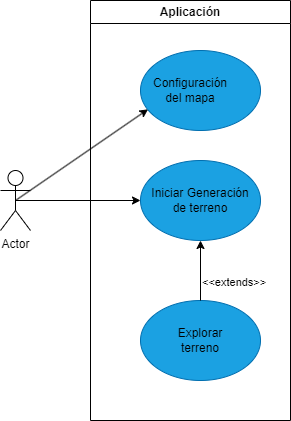
\includegraphics[width=0.5\textwidth]{img/UseCases.png}
    \caption{Diagrama de Casos de Uso del Proyecto.}
\end{figure}


El diagrama de secuencia detallará las interacciones entre los componentes del sistema, incluidos el \texttt{MapGenerator}, el \texttt{MeshGenerator}, el \texttt{EndlessTerrain}, y otros, durante la generación y visualización del terreno.

\begin{figure}[H]
    \centering
    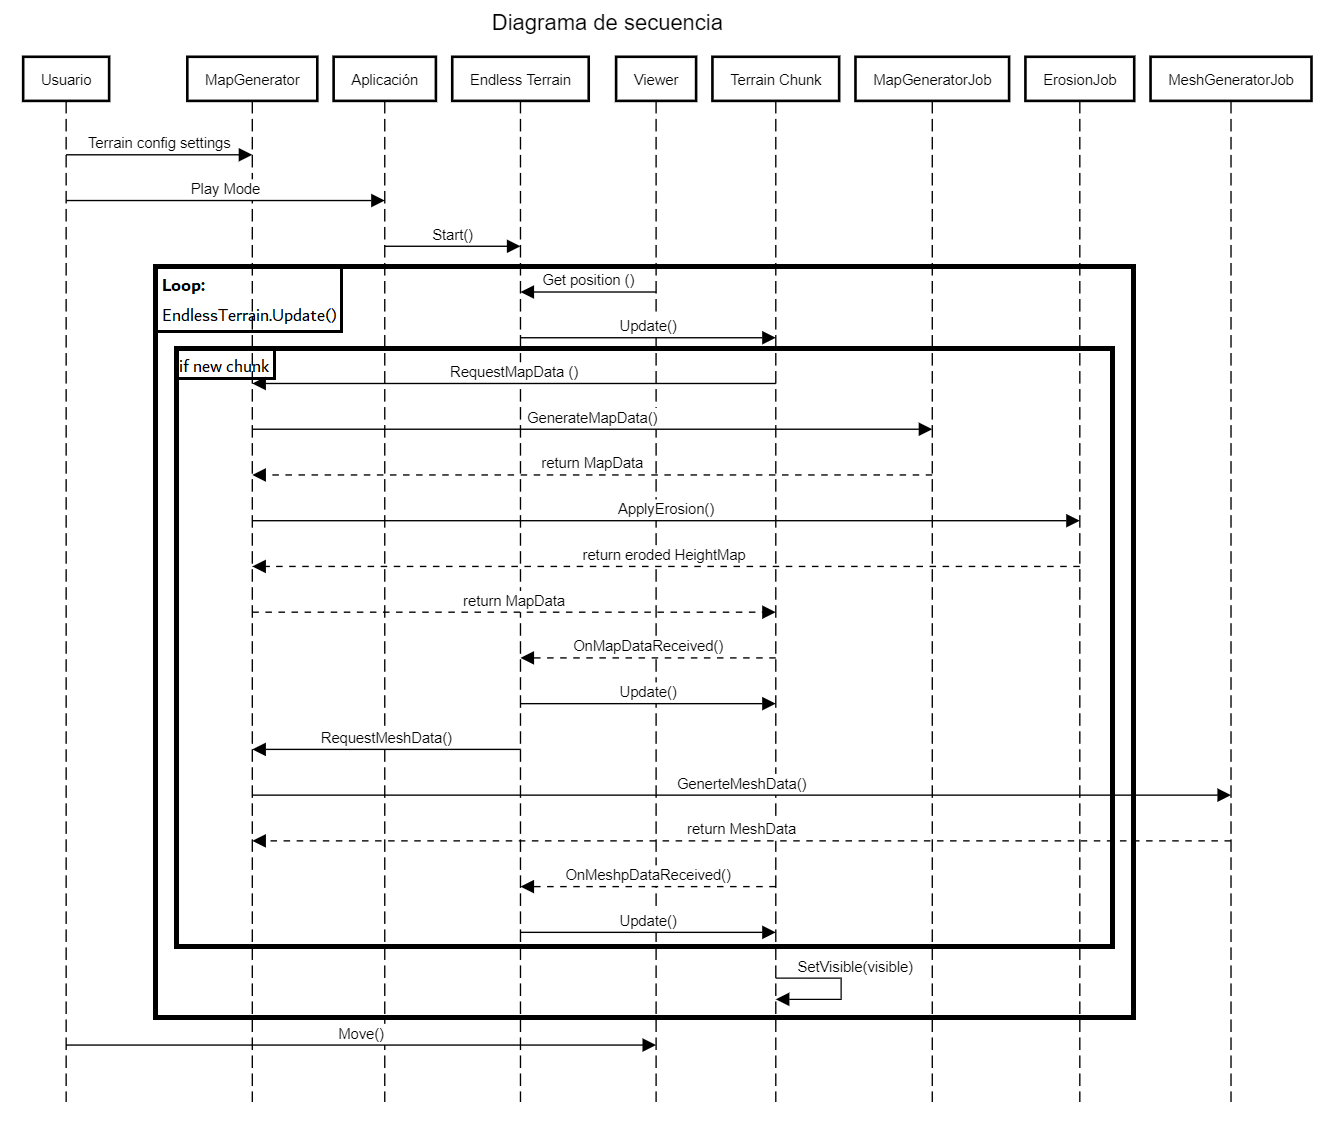
\includegraphics[width=1\textwidth]{img/Diagrama de secuencia.png}
    \caption{Diagrama de Secuencia de Generación de Terreno.}
\end{figure}


\subsection{Tecnologías y Herramientas Utilizadas}

\subsubsection{Elección de Tecnologías}
La elección de las tecnologías específicas para este proyecto se basó en los siguientes criterios:

\begin{itemize}
    \item \textbf{Unity 3D:} Se eligió Unity como motor de desarrollo debido a su versatilidad y capacidad para crear aplicaciones interactivas en 3D. Unity proporciona una amplia gama de herramientas y recursos que facilitan el desarrollo de juegos y simulaciones.
    
    \item \textbf{Unity Job System:} Para optimizar el rendimiento en la generación de terrenos, se utiliza el Unity Job System, que permite la paralelización de tareas en múltiples núcleos de CPU.
    
    \item \textbf{Burst Compiler:} La herramienta Burst Compiler se utiliza para compilar el código C \# en código nativo altamente optimizado, mejorando aún más el rendimiento de la generación de terrenos.
    
    \item \textbf{Perlin Noise, Voronoi y Simplex Noise:} Se implementan algoritmos de ruido Perli, Simplex y Voronoi para la generación de terrenos. Estos algoritmos proporcionan resultados realistas y variados.
    
\end{itemize}

Estas tecnologías se eligieron cuidadosamente para garantizar un rendimiento óptimo y una alta calidad en la generación de terrenos en tiempo real.

\subsubsection{Lenguajes de Programación}
\begin{itemize}
    \item \textbf{C\#:} Este proyecto está programado enteramente utilizando C\# como lenguaje de programación. C\# es el lenguaje que utilizan los componentes Scripts de Unity por lo que está altamente integrado con el motor, y es un lenguaje orientado a objetos que ofrece un alto rendimiento y facilidad de uso.
    
\end{itemize}

\subsubsection{Herramientas de Desarrollo}

Durante el desarrollo de este proyecto, se utilizaron diversas herramientas y software que desempeñaron un papel fundamental en la planificación, implementación y gestión del trabajo. A continuación, se detallan las principales herramientas de desarrollo utilizadas:

\begin{itemize}
    \item \textbf{IDE Principal:} JetBrains Rider fue el IDE principal utilizado para el desarrollo en C\#. Rider proporcionó un entorno de desarrollo integrado eficiente y potente para la escritura de código, depuración y pruebas del proyecto.
    
    \item \textbf{Visual Studio:} Visual Studio se utilizó específicamente para la creación de diagramas de clases, lo que permitió una representación visual clara de la estructura del proyecto y las relaciones entre las clases.
    
    \item \textbf{VS Code:} Visual Studio Code, junto con el plugin draw.io, se utilizó para crear varios tipos de diagramas, incluidos los diagramas de casos de uso y diagramas de flujo. Estas representaciones gráficas ayudaron a comprender y comunicar el flujo de trabajo del sistema. También se suó para la redacción en Latex de la memoria.
        
    \item \textbf{Control de Versiones (Git y GitHub):} Git se utilizó para el control de versiones del código fuente del proyecto. GitHub se empleó como plataforma de alojamiento para el repositorio de Git, lo que facilitó la colaboración en equipo y el seguimiento de cambios.
    
    \item \textbf{Gestión de Tareas (Trello):} Trello se utilizó para la gestión de tareas y la planificación del proyecto. La herramienta permitió organizar y priorizar tareas, así como realizar un seguimiento del progreso de cada elemento del proyecto.
    
    \item \textbf{Burst Compiler:} El Burst Compiler se utilizó para compilar el código C\# en código nativo altamente optimizado, lo que contribuyó significativamente a mejorar el rendimiento en la generación de terrenos.
\end{itemize}

Estas herramientas desempeñaron un papel esencial en la realización exitosa del proyecto, proporcionando las capacidades necesarias para el desarrollo, la documentación, la colaboración en equipo y la optimización de rendimiento.

\subsubsection{Alternativas Consideradas}
Antes de tomar las decisiones de diseño finales, se consideraron varias alternativas, incluyendo:

\begin{itemize}
    \item \textbf{Otras Tecnologías de Generación de Terrenos:} Se evaluaron diferentes tecnologías y enfoques para la generación de terrenos, como el uso de mapas de altura pregenerados versus generación procedural en tiempo real.
    
    \item \textbf{Métodos de Optimización:} Se exploraron diversas técnicas de optimización además del Unity Job System, como el uso de GPU para cálculos intensivos o la paralelización mediante threads manual.
    
    \item \textbf{Otros Algoritmos de Ruido:} Se investigaron algoritmos de ruido alternativos además de Perlin y Simplex para determinar cuáles producirían los resultados deseados y técnicas de generación, como el algoritmo diamante-cuadrado. Pero se optó por el ruido debido a que facilitaba la consistencia entre lso bordes de partes de terreno nuevas generadas
\end{itemize}

\subsection{Planificación del Desarrollo}

\subsubsection{Metodología de Desarrollo}
El proyecto siguió una metodología de desarrollo ágil, lo que permitió una adaptación flexible a medida que se abordaban desafíos técnicos y se tomaban decisiones de diseño. Se realizaron reuniones periódicas de revisión y planificación para ajustar el enfoque según fuera necesario. Cada día se fueron subiendo incrementos de desarrollo al repositorio remoto, gestioando un control de cuáles habían sido las mejroas subidas, cuál era el estado del proyecto y cuáles debían ser los siguientes objetivos.

\subsubsection{Gestión de Tiempo}
La gestión del tiempo se realizó mediante una planificación detallada en Trello. Creando pilas de tareas "por hacer", "en desarrollo", "termiandas" y "mejorables".

La planificación del proyecto se ha desglosado en las siguientes fases, las cuales culminan con sus correspondientes hitos.
\begin{itemize}
    \item Análisis preeliminar: Esta fase es en la que se determinan los objetivos, los requisitos, alcance del proyecto y se hace una investigación sobre los recursos que se pueden emplear para el proyecto. Esta fase culmina con el hito de la aprobación del análsis preeliminar.
    \item Fase de Análisis: Esta fase corresponde como su propio nombre indica al análisis del proyecto: estudio de requisitos, de la arquitectura que se va a diseñar y de los procesos y componentes necesarios para el proyecto. esta fase culmina.Esta fase culmina con el hito de la aprobación del análsis.
    \item Fase de Diseño: En la fase de diseño se diseñará la estructura de la arquitectura que tendrá la herramienta, los componentes y relaciones entre ellos, así como los parámetros que tendrá de el ususrio para configurar la generación de terreno. Esta fase culmina con la aprobcación del diseño.
    \item Implementación: Durante la implementación se implementan todos los compoentnes, clases y procesos necesarios. Culmina con el finde la implementación y comienzo de las pruebas.
    \item Pruebas y resutlados: Aquí se desarrollan diferentes pruebasy correcciones sobre la implementación anterior. Esta fase culmina con la aprobación de los resutladso de las últimas pruebas que se realicen.
    \item Finalización de la documentación: El hito de la finalización de la documentación culmina con la entrega de la memoria y el video explicativo de este proyecto.
\end{itemize}

El cronograma de desarrollo detallado se encuentra en el apéndice A para una referencia más completa.

\subsubsection{Recursos Necesarios}
Los recursos necesarios para llevar a cabo el desarrollo incluyeron:

\begin{itemize}
    \item Personal de Desarrollo: Para este proyecto el personal fue una única persona que ocupó todos los roles del desarrollo y un product owner que especificaba los requisitos que debía cumplir el proyecto.
    
    \item Hardware: Se utilizó un equipo portátil con procesador i5-11400H con 2.7GHz, 16 GB de RAM, 1TB de memoria en disco y tarjeta gráfica NVidia 3060 con 6GB de RAM. El equipo contaba con windows 10 Home como sistema operativo. 
    
    \item Software: Se requirieron herramientas como Unity3D, JetBrains Rider, Visual Studio, VS Code con el plugin draw.io, LaTeX y el Burst Compiler para el desarrollo y la documentación del proyecto.
\end{itemize}



\chapter{Diseño}
% Contenidos del capítulo.
% Las secciones presentadas son orientativas y no representan
% necesariamente la organización que debe tener este capítulo.

% Diagramas de clases, de secuencia, de despliegue, diseño de
% pantallas, etc


\chapter{Implementación y pruebas}
\section{Implementación}

En esta sección, se detalla la implementación del sistema de generación de terreno procedural en Unity. Se describe en profundidad la estructura de la herramienta, la implementación de los algoritmos y la resolución de problemas encontrados durante el desarrollo.

\subsection{Implementación de la Arquitectura}

En esta subsección, se aborda la implementación detallada de la estructura de la herramienta en Unity. Se describen los scripts y la organización de los componentes que conforman la arquitectura del sistema.

\subsubsection{Scripts y Componentes Clave}

Se presentan y explican los scripts y componentes clave que forman parte de la arquitectura del sistema, incluyendo su función y relación con otros elementos.

\begin{enumerate}
    \item \textbf{EndlessTerrain}:
    La clase \texttt{EndlessTerrain} es la clase de unity que implementa la generación de chunks de terreno infinita, la cual se ha traducido en código de la siguiente forma.

    Consta de los siguientes \texttt{atributos:}

    \begin{itemize}
        \item \texttt{Scale}: Escala utilizada para ajustar la posición del terreno.
        \item \texttt{ViewerMoveThresholdForChunkUpdate}: Umbral de movimiento del espectador para actualizar chunks.
        \item \texttt{SqrViewerMoveThresholdForChunkUpdate}: Umbral de movimiento al cuadrado.
        \item \texttt{detailLevels}: Niveles de detalle (LOD) del terreno.
        \item \texttt{ maxViewDst}: Máxima distancia de visualización.
        \item \texttt{viewer}: Transform del espectador.
        \item \texttt{ mapMaterial}: Material del mapa.
        \item \texttt{viewerPosition}: Posición del espectador.
        \item \texttt{\_viewerPositionOld}: Posición anterior del espectador.
        \item \texttt{\_mapGenerator}: Instancia del generador de mapas.
        \item \texttt{\_chunkSize}: Tamaño de los chunks del mapa.
        \item \texttt{\_chunksVisibleInViewDst}: Cantidad de chunks visibles en la distancia.
        \item \texttt{\_terrainChunkDictionary}: Diccionario que almacena los chunks de terreno.
        \item \texttt{\_terrainChunksVisibleLastUpdate}: Lista de chunks visibles en la última actualización.
    \end{itemize}

    \texttt{Métodos Principales}

    \begin{itemize}
        \item \texttt{void Start()}: Inicializa la clase.
        \item \texttt{void Update()}: Actualiza la posición del espectador y gestiona la actualización de chunks.
        \item \texttt{void UpdateVisibleChunks()}: Actualiza la visibilidad de los chunks de terreno en función de la posición del espectador.
    \end{itemize}

    \texttt{Funcionalidad:}

    En la subseccion \ref{subsec:generacion-infinita} se profundiza en el método en que se genera el terrneo infinito.\\
    \\

    \item \textbf{TerrainChunk}:

    La clase \texttt{TerrainChunk} es la encargada de representar y gestionar un chunk de terreno individual en Unity. A continuación, se detallan sus atributos y métodos clave:

    \texttt{Atributos:}

    \begin{itemize}
        \item \texttt{\_meshObject}: Objeto de juego que representa el chunk de terreno.
        \item \texttt{\_position}: Posición del chunk en coordenadas locales.
        \item \texttt{\_bounds}: Área delimitada que abarca el chunk.
        \item \texttt{\_meshRenderer}: Componente para la representación visual del terreno.
        \item \texttt{\_meshFilter}: Componente para gestionar la malla del terreno.
        \item \texttt{\_meshCollider}: Componente para las colisiones del terreno.
        \item \texttt{\_detailLevels}: Niveles de detalle (LOD) disponibles.
        \item \texttt{\_lodMeshes}: Array de objetos LODMesh para cada nivel de detalle.
        \item \texttt{\_mapData}: Datos del mapa asociados a este chunk.
        \item \texttt{\_mapDataReceived}: Indica si los datos del mapa han sido recibidos.
        \item \texttt{\_previousLODIndex}: Índice del nivel de detalle (LOD) previamente utilizado.
    \end{itemize}

    \texttt{Métodos Principales:}

    \begin{itemize}
        \item \texttt{TerrainChunk(Vector2 coord,  size, LODInfo[] detailLevels, Transform parent, Material material)}: Constructor de la clase que inicializa un chunk de terreno.
        \item \texttt{void OnMapDataReceived(MapData mapData)}: Callback llamado cuando se reciben los datos del mapa.
        \item \texttt{void UpdateTerrainChunk()}: Actualiza la visibilidad y el nivel de detalle del chunk.
        \item \texttt{void SetVisible(bool visible)}: Establece la visibilidad del chunk.
        \item \texttt{bool IsVisible()}: Verifica si el chunk es visible.
    \end{itemize}

    \texttt{Funcionalidad:}

    La clase \texttt{TerrainChunk} es responsable de representar un chunk específico del terreno. Cuando se crea un objeto de esta clase, se inicializa con sus atributos y se solicitan los datos del mapa asociados a ese chunk. Luego, durante la actualización, se verifica si el chunk debe ser visible en función de su distancia al espectador y se ajusta su nivel de detalle (LOD) en consecuencia. Finalmente, se gestiona la visibilidad del chunk y su representación visual.\\
    \\

    \item \textbf{LODMesh}:

    La clase \texttt{LODMesh} se encarga de gestionar las mallas de diferentes niveles de detalle (LOD) utilizadas en la representación del terreno. Aquí se detallan sus atributos y métodos clave:

    \texttt{Atributos:}

    \begin{itemize}
        \item \texttt{mesh}: Representa la malla del terreno para un nivel de detalle (LOD) específico.
        \item \texttt{hasRequestedMesh}: Indica si se ha solicitado la generación de la malla.
        \item \texttt{hasMesh}: Indica si la malla está disponible.
        \item \texttt{\_lod}: Nivel de detalle (LOD) asociado a esta malla.
        \item \texttt{\_updateCallback}: Callback que se llama cuando se recibe la malla.
    \end{itemize}

    \texttt{Métodos Principales:}

    \begin{itemize}
        \item \texttt{void OnMeshDataReceived(MeshData meshData)}: Callback llamado cuando se reciben los datos de la malla.
        \item \texttt{void RequestMesh(MapData mapData)}: Solicita la generación de la malla asociada a este LOD.
    \end{itemize}

    \texttt{Funcionalidad:}

    La clase \texttt{LODMesh} gestiona las mallas correspondientes a diferentes niveles de detalle del terreno. Cuando se crea un objeto de esta clase, se establece el nivel de detalle (LOD) y un callback que se ejecutará cuando la malla esté disponible. La función \texttt{RequestMesh} inicia la solicitud de generación de la malla.\\
    \\

    \item \textbf{LODInfo}:

    La estructura \texttt{LODInfo} almacena información sobre los niveles de detalle (LOD) utilizados para optimizar la representación del terreno. A continuación, se detallan sus atributos:

    \texttt{Atributos:}

    \begin{itemize}
        \item \texttt{lod}: Representa el nivel de detalle (LOD).
        \item \texttt{visibleDstThreshold}: Define la distancia a la que se activa este nivel de detalle.
    \end{itemize}

    \texttt{Funcionalidad:}

    La estructura \texttt{LODInfo} se utiliza para configurar los niveles de detalle (LOD) y establecer los umbrales de distancia a los cuales se activa cada nivel. Esto permite optimizar la representación del terreno en función de la proximidad al espectador.\\
    \\
 
    \item \textbf{MapGenerator}:

    La clase \texttt{MapGenerator} es responsable de generar y gestionar los datos del mapa, así como de generar mallas de terreno en Unity. A continuación, se describen sus atributos y métodos clave:

    \texttt{Atributos:}

    \begin{itemize}
        \item \texttt{ MapChunkSize}: Tamaño de los chunks del mapa.
        \item \texttt{configSettings}: Configuración del generador de mapas.
        \item \texttt{colorGradient}: Gradiente de colores utilizado para asignar colores al terreno.
        \item \texttt{\_batchSize}: Tamaño del lote para las operaciones en paralelo.
    \end{itemize}

    \texttt{Métodos Principales:}

    \begin{itemize}
        \item \texttt{void DrawMapInEditor()}: Dibuja el mapa en el editor de Unity.
        \item \texttt{void RequestMapData(Vector2 centre, Action<MapData> callback)}: Solicita datos del mapa en una ubicación específica y llama a un callback cuando los datos están listos.
        \item \texttt{void RequestMeshData(MapData mapData,  lod, Action<MeshData> callback)}: Solicita datos de malla del terreno y llama a un callback cuando la malla está lista.
    \end{itemize}

    \texttt{Funcionalidad:}

    La clase \texttt{MapGenerator} se encarga de generar datos del mapa y mallas de terreno en función de la configuración proporcionada. Puede generar mapas de ruido, mapas de colores y mallas de terreno. Los métodos \texttt{RequestMapData} y \texttt{RequestMeshData} permiten solicitar estos datos y mallas de manera asincrónica.

    Además, la clase realiza la erosión del terreno si la configuración así lo indica, aplicando un número específico de ciclos de erosión al mapa de alturas.

    También se encarga de la generación de mallas de terreno a diferentes niveles de detalle (LOD) utilizando el sistema de jobs de Unity para un rendimiento óptimo.\\
    \\

    \item \textbf{MapData}:

    La estructura \texttt{MapData} almacena los datos generados del mapa, incluido el mapa de alturas y el mapa de colores. A continuación, se describen sus atributos:

    \texttt{Atributos:}

    \begin{itemize}
        \item \texttt{[] heightMap}: Mapa de alturas del terreno.
        \item \texttt{Color[] colourMap}: Mapa de colores del terreno.
    \end{itemize}

    \texttt{Funcionalidad:}

    La estructura \texttt{MapData} proporciona una forma de encapsular y transportar los datos generados del mapa entre diferentes partes del programa. Almacena tanto el mapa de alturas como el mapa de colores para su uso en la representación del terreno.\\
    \\

    \item \textbf{MapDataGeneratorJob}:

    La estructura \texttt{MapDataGeneratorJob} representa un trabajo en paralelo utilizado para generar datos del mapa, incluyendo el mapa de alturas y el mapa de colores del terreno. A continuación, se describen sus atributos y métodos clave:

    \texttt{Atributos:}

    \begin{itemize}
        \item \texttt{\_heightMap}: Un array nativo que almacena el mapa de alturas del terreno.
        \item \texttt{\_colMap}: Un array nativo que almacena el mapa de colores del terreno.
        \item \texttt{\_heightMapSettings}: Configuración de generación del mapa de alturas, que incluye detalles como octavas, frecuencia y amplitud.
        \item \texttt{\_mapChunkSize}: El tamaño del chunk del mapa.
        \item \texttt{\_centre}: El centro del mapa en coordenadas 2D.
        \item \texttt{\_colorGradient}: Un array nativo que almacena una paleta de colores utilizada para mapear alturas a colores.
    \end{itemize}

    \texttt{Métodos Principales:}

    \begin{itemize}
        \item \texttt{MapDataGeneratorJob(HeightMapSettings heightMapSettings, \\int mapChunkSize, float2 centre, NativeArray<Color> colorGradient)}: Constructor de la estructura \texttt{MapDataGeneratorJob} que recibe la configuración del mapa de alturas, el tamaño del chunk del mapa, el centro del mapa y la paleta de colores.

        \item \texttt{Execute(int threadIndex)}: Método que se ejecuta en paralelo para generar datos del mapa en una posición específica. Calcula la altura en esa posición y asigna un color correspondiente basado en la paleta de colores.

        \item \texttt{ReturnMapData()}: Método que devuelve los datos generados del mapa, incluyendo el mapa de alturas y el mapa de colores, en forma de una estructura \texttt{MapData}.

        \item \texttt{Dispose()}: Método que se encarga de liberar los recursos utilizados por los arrays nativos \texttt{\_colMap} y \texttt{\_heightMap} una vez que se han generado los datos del mapa.

    \end{itemize}

    La estructura \texttt{MapDataGeneratorJob} es esencial en el proceso de generación de terreno, ya que calcula y asigna alturas y colores a cada punto del mapa en paralelo, lo que permite una generación eficiente del terreno.\\
    \\

    \item \textbf{Noise}:

    La clase `Noise` es una utilidad que proporciona métodos para generar mapas de ruido, que se utilizan en la generación de terrenos. Esta clase contiene una enumeración `Type` que define los tipos de ruido disponibles, como Perlin, Simplex y Voronoi.

    \texttt{Métodos Principales:}

    \begin{itemize}
        \item \texttt{GenerateNoiseMap(int mapSize, HeightMapSettings parameters, float2 centre)}: Este método genera un mapa de ruido basado en parámetros dados, como el tamaño del mapa, la configuración de mapas de alturas y el centro del mapa. Utiliza el ruido Perlin para calcular alturas y devuelve un array de floats que representa el mapa de ruido generado.

        \item \texttt{GenerateNoiseValue(float2 position, HeightMapSettings parameters)}: Este método genera un valor de ruido en una posición dada utilizando los parámetros de configuración y la posición proporcionada. Puede utilizar diferentes tipos de ruido según los parámetros. Devuelve un valor de ruido float en función de la posición.

        \item \texttt{SampleNoiseValue(float2 sample, Type type)}: Este método toma una muestra de ruido en una posición dada utilizando el tipo de ruido especificado. Puede ser Perlin, Simplex o Voronoi. Devuelve un valor de ruido float en función del tipo de ruido y la posición de la muestra.

    \end{itemize}

    La clase `Noise` es esencial en la generación de terrenos, ya que proporciona las herramientas para generar mapas de ruido que se utilizan para determinar las alturas y características del terreno, lo que contribuye a la variedad y realismo del entorno generado.\\
    \\

    \item \textbf{MeshGenerator}:

    La clase \texttt{MeshGenerator} es una clase estática que se encarga de generar las mallas de terreno para el sistema de generación de terreno en Unity. A continuación, se describen sus atributos y métodos clave:

    \texttt{Métodos Principales:}

    \begin{itemize}
        \item \texttt{ MeshData GenerateTerrainMesh([] heightMap, MeshSettings parameters,  size,  levelOfDetail)}: Genera una malla de terreno a partir de un mapa de alturas y una configuración dada. Esta función calcula los vértices, triángulos y coordenadas UV de la malla en función de los parámetros proporcionados.

        \texttt{Atributos:}

        \begin{itemize}
            \item \texttt{topLeftX}: Coordenada X del vértice superior izquierdo del terreno.
            \item \texttt{topLeftZ}: Coordenada Z del vértice superior izquierdo del terreno.
            \item \texttt{meshSimplificationIncrement}: Incremento de simplificación de malla para LOD.
            \item \texttt{verticesPerLine}: Número de vértices por línea en la malla.
            \item \texttt{MeshData meshData}: Objeto que almacena los datos de la malla, incluyendo vértices, triángulos y coordenadas UV.
            \item \texttt{vertexIndex}: Índice actual del vértice.
        \end{itemize}

        Esta función recorre el mapa de alturas y genera los vértices de la malla en función de la altura de cada punto en el mapa. También calcula los triángulos que forman la malla y las coordenadas UV para mapear texturas.
    \end{itemize}

    La clase \texttt{MeshGenerator} es esencial para la generación de mallas de terreno y su adaptación a diferentes niveles de detalle (LOD) en el sistema de generación de terreno en Unity.\\
    \\

    \item \textbf{MeshData}: Esta estructura almacena los datos de una malla de terreno, incluyendo los vértices, triángulos, coordenadas UV y un índice de triángulo actual.

    \texttt{Atributos:}

    \begin{itemize}
        \item \texttt{vertices}: Array de vectores que representan los vértices de la malla.
        \item \texttt{triangles}: Array de enteros que define los triángulos de la malla.
        \item \texttt{uvs}: Array de vectores 2D que almacena las coordenadas UV de la malla.
        \item \texttt{triangleIndex}: Índice actual de triángulo.
    \end{itemize}

    \texttt{Funcionalidad:}

    La estructura \texttt{MeshData} proporciona una forma de almacenar y transportar los datos de una malla de terreno. Además, incluye un método para añadir triángulos y otro para crear una malla Unity a partir de los datos almacenados.\\
    \\

    \item \textbf{MeshDataGeneratorJob}:

    La estructura \texttt{MeshDataGeneratorJob} representa un trabajo en paralelo utilizado para generar datos de malla para el terreno. Su objetivo principal es calcular las coordenadas de vértices, coordenadas UV y triángulos de la malla del terreno en función de un mapa de alturas. A continuación, se describen sus atributos y métodos clave:

    \texttt{Atributos:}

    \begin{itemize}
        \item \texttt{\_size}: El tamaño de la malla.
        \item \texttt{\_meshSimpplificationIncrement}: El incremento de simplificación de la malla.
        \item \texttt{\_meshSettings}: Configuración de la malla, que incluye detalles como la altura del agua.
        \item \texttt{\_heightMap}: Un array nativo que almacena el mapa de alturas del terreno.
        \item \texttt{\_vertices}: Un array nativo que almacena las coordenadas de los vértices de la malla.
        \item \texttt{\_uvs}: Un array nativo que almacena las coordenadas UV de la malla.
        \item \texttt{\_triangles}: Un array nativo que almacena la información de los triángulos de la malla.
    \end{itemize}

    \texttt{Métodos Principales:}

    \begin{itemize}
        \item \texttt{MeshDataGeneratorJob(int size, int meshSimplificationIncrement, \\MeshSettings meshSettings, NativeArray<float> heightMap, NativeArray<Vector3> \\vertices, NativeArray<Vector2> uvs, NativeArray<int> triangles)}: Constructor de la estructura \texttt{MeshDataGeneratorJob} que recibe el tamaño de la malla, el incremento de simplificación de la malla, la configuración de la malla, el mapa de alturas, y los arrays nativos para almacenar los datos de la malla.

        \item \texttt{Execute(int index)}: Método que se ejecuta en paralelo para calcular las coordenadas de vértices, coordenadas UV y triángulos de la malla en función de la información del mapa de alturas. Cada hilo de trabajo calcula estos datos para una posición específica en la malla.

    \end{itemize}

    La estructura \texttt{MeshDataGeneratorJob} es esencial en el proceso de generación de la malla del terreno, ya que permite calcular eficientemente las coordenadas de vértices y triángulos, lo que resulta en un terreno visualmente atractivo y detallado.\\
    \\

    \item \textbf{Erosion}:

    La clase \texttt{Erosion} es una clase estática que implementa el proceso de erosión térmica en el contexto del sistema de generación de terreno en Unity. A continuación, se describen sus atributos y métodos clave:

    \texttt{Métodos Principales:}

    \begin{itemize}
        \item \texttt{public static float ThermalErosionValue(int x, int y, int mapChunkSize, ErosionSettings erosionSettings, NativeArray<float> heightMap, float iterFraction)}: Este método calcula el valor erosionado de una posición dada en el mapa de alturas utilizando el proceso de erosión térmica.

        \texttt{Parámetros:}

        \begin{itemize}
            \item \texttt{x, y}: Coordenadas de la posición en el mapa de alturas.
            \item \texttt{mapChunkSize}: Tamaño del chunk del mapa.
            \item \texttt{erosionSettings}: Configuración de erosión que incluye valores como el tamaño del borde y el ángulo de talud.
            \item \texttt{heightMap}: Array nativo que almacena el mapa de alturas.
            \item \texttt{iterFraction}: Fracción de iteración actual (para controlar la erosión en cada iteración).
        \end{itemize}

        Este método calcula el efecto de la erosión térmica en la altura del terreno en una posición específica. Compara la altura actual con la altura de los vecinos y ajusta la altura según el ángulo de talud y la configuración de erosión.

        \item \texttt{private static bool InsideBorder(int x, int y, int borderSize, int mapChunkSize)}: Este método verifica si una posición dada está dentro del área del borde definida por el tamaño del borde.

        \texttt{Parámetros:}

        \begin{itemize}
            \item \texttt{x, y}: Coordenadas de la posición en el mapa de alturas.
            \item \texttt{borderSize}: Tamaño del borde.
            \item \texttt{mapChunkSize}: Tamaño del chunk del mapa.
        \end{itemize}

        Este método se utiliza para determinar si una posición dada está dentro del área del borde, lo que afecta a la aplicación de la erosión térmica en esa posición.

    \end{itemize}

    La clase \texttt{Erosion} desempeña un papel importante en el proceso de generación de terreno, específicamente en la simulación de la erosión térmica que afecta a la topografía del terreno generado.\\
    \\

    \item \textbf{ErosionJob}:

    La estructura \texttt{ErosionJob} representa un trabajo en paralelo que se encarga de aplicar la erosión térmica al mapa de alturas de un terreno. A continuación, se describen sus atributos y métodos clave:

    \texttt{Atributos:}

    \begin{itemize}
        \item \texttt{\_heightMap}: Un array nativo de solo lectura que almacena el mapa de alturas original.
        \item \texttt{\_erodedHeightMap}: Un array nativo que almacena el resultado de la erosión térmica.
        \item \texttt{\_mapChunkSize}: El tamaño del chunk del mapa.
        \item \texttt{\_erosionSettings}: Configuración de erosión que incluye valores como el tamaño del borde y el ángulo de talud.
        \item \texttt{\_iterFraction}: Fracción de iteración actual (para controlar la erosión en cada iteración).
    \end{itemize}

    \texttt{Métodos Principales:}

    \begin{itemize}
        \item \texttt{public ErosionJob(NativeArray<float> heightMap, ErosionSettings \\erosionSettings, int mapChunkSize, float iterFraction)}: Constructor de la estructura \texttt{ErosionJob} que recibe el mapa de alturas original, la configuración de erosión, el tamaño del chunk del mapa y la fracción de iteración actual.

        \texttt{Parámetros:}

        \begin{itemize}
            \item \texttt{heightMap}: Un array nativo que almacena el mapa de alturas original.
            \item \texttt{erosionSettings}: Configuración de erosión que incluye valores como el tamaño del borde y el ángulo de talud.
            \item \texttt{mapChunkSize}: Tamaño del chunk del mapa.
            \item \texttt{iterFraction}: Fracción de iteración actual (para controlar la erosión en cada iteración).
        \end{itemize}

        Este constructor inicializa los atributos de la estructura y crea un nuevo array nativo para almacenar el mapa de alturas erosionado.

        \item \texttt{public void Execute(int threadIndex)}: Método que se ejecuta en paralelo para calcular y aplicar la erosión térmica en una posición específica del mapa de alturas.

        \texttt{Parámetros:}

        \begin{itemize}
            \item \texttt{int threadIndex}: Índice del hilo de ejecución que indica la posición en el mapa de alturas.
        \end{itemize}

        Este método utiliza la función \texttt{Erosion.ThermalErosionValue()} para calcular la erosión en una posición dada y almacena el valor erosionado en el array nativo \texttt{\_erodedHeightMap}.

        \item \texttt{public NativeArray<float> GetErodedHeightMap()}: Método que devuelve el array nativo que contiene el mapa de alturas erosionado.

        \item \texttt{public void Dispose()}: Método que se encarga de liberar los recursos utilizados por el array nativo \texttt{\_erodedHeightMap} una vez que la erosión ha sido aplicada.

    \end{itemize}

    La estructura \texttt{ErosionJob} es fundamental en el proceso de simulación de erosión térmica en el terreno, ya que realiza cálculos paralelos para actualizar el mapa de alturas con los efectos de la erosión.\\
    \\
    \item \textbf{ConfigSettings}:

    La estructura `ConfigSettings` contiene configuraciones generales para la generación de terrenos en Unity. Estas configuraciones se utilizan para controlar aspectos como la vista previa en el editor, las configuraciones del mapa de alturas, la erosión del terreno y las opciones de malla.

    \texttt{Componentes Principales:}

    \begin{itemize}
        \item \texttt{editorPreviewSettings}: Un componente que almacena configuraciones relacionadas con la vista previa en el editor, como el modo de dibujo y la actualización automática.
        
        \item \texttt{heightMapSettings}: Un componente que almacena configuraciones relacionadas con el mapa de alturas, como el tipo de ruido, la escala del ruido y la semilla de generación.
        
        \item \texttt{erosionSettings}: Un componente que almacena configuraciones relacionadas con la erosión del terreno, como la activación de la erosión, la cantidad de ciclos y otros parámetros relacionados con el borde y el ángulo de talud.
        
        \item \texttt{meshSettings}: Un componente que almacena configuraciones relacionadas con la malla de terreno, como el multiplicador de altura de la malla, el nivel del agua y el nivel de detalle de la vista previa en el editor.
    \end{itemize}

    La estructura `ConfigSettings` es esencial para personalizar y controlar cómo se genera y se visualiza el terreno en Unity. Cada componente almacena configuraciones específicas que afectan diferentes aspectos de la generación y visualización del terreno.
\end{enumerate}

\subsection{Implementación de los Algoritmos}

En esta subsección, se profundiza en la implementación de los algoritmos de generación procedimental de terrenos en Unity. Se incluye el código utilizado y se explican las decisiones específicas de implementación.

\subsubsection{Generación Infinita de Chunks de Terreno}

\textbf{Inicio de la generación:}\label{subsec:generacion-infinita}

\begin{itemize}
    \item \textbf{Distancia de Visibilidad}: Se calcula la distancia a la que los chunks serán visibles para el jugador.
    \item \textbf{Tamaño del Chunk}: Se determina el tamaño de cada chunk que se generará.
    \item \textbf{Número de Chunks Visibles}: Se calcula el número de chunks que serán visibles en función de la distancia de visibilidad y el tamaño del chunk.
    \item \textbf{Actualización de chunks visibles}: Se generan los primeros chunks visibles
\end{itemize}
\begin{figure}[h]
    \centering
    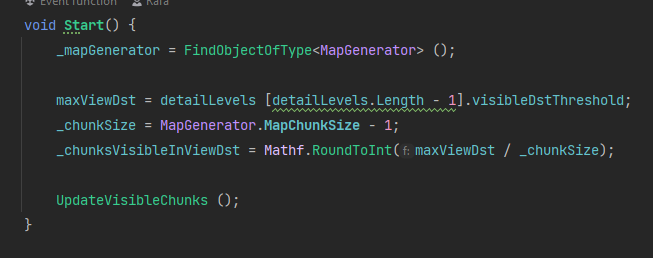
\includegraphics[width=1\textwidth]{img/codes/EndlessTerrain-start.png}
    \caption{Inicialización de parámetros para generación de terreno infinito.}
\end{figure}

\textbf{Actualización de chunks visibles:}

La Actualización de chunks visibles se realiza en la función \texttt{UpdateVisibleChunks} y es donde se gestiona la visibilidad de los chunks de terreno en función de la posición del jugador y se actualizan los chunks que deben estar visibles en la escena.

Para ello esta función realiza los siguientes pasos:

\begin{enumerate}
    \item Recorre la lista \texttt{\_terrainChunksVisibleLastUpdate}, que es una lista de chunks de terreno que estaban visibles en la actualización anterior. Dentro del bucle, se llama al método \texttt{SetVisible(false)} en cada chunk para ocultarlos.
    \item Después de ocultar todos los chunks visibles en la actualización anterior, se borra la lista \texttt{\_terrainChunksVisibleLastUpdate}, preparándola para su uso en la próxima actualización.
    \item Se calculan las coordenadas del chunk actual en el que se encuentra el jugador. Esto se hace dividiendo las coordenadas X e Y de la posición del jugador (\texttt{viewerPosition}) por el tamaño de un chunk (\texttt{\_chunkSize}) y redondeando los resultados a números enteros.
    \item Se inician dos bucles anidados, uno para \texttt{yOffset} (variando desde \\\texttt{-\_chunksVisibleInViewDst} hasta \texttt{\_chunksVisibleInViewDst}) y otro para \texttt{xOffset} (también variando desde \texttt{-\_chunksVisibleInViewDst} hasta \texttt{\_chunksVisibleInViewDst}). Esto se hace para recorrer los chunks en un área cuadrada alrededor del jugador, determinada por \texttt{\_chunksVisibleInViewDst}.
    \item Dentro de los bucles anidados, se calcula \texttt{viewedChunkCoord}, que representa las coordenadas del chunk que se está evaluando actualmente en función de la posición actual del jugador y los desplazamientos \texttt{xOffset} e \texttt{yOffset}.
    \item Luego, se verifica si el diccionario \texttt{\_terrainChunkDictionary} contiene una entrada con las coordenadas \texttt{viewedChunkCoord}. Si existe, significa que el chunk ya ha sido creado previamente, por lo que se llama al método \texttt{UpdateTerrainChunk} en ese chunk para actualizar su visualización en función de la distancia al jugador.
    \item Si no existe una entrada en el diccionario para las coordenadas \texttt{viewedChunkCoord}, significa que el chunk aún no se ha creado. En este caso, se crea un nuevo objeto \texttt{TerrainChunk} con las coordenadas \texttt{viewedChunkCoord}, el tamaño del chunk \texttt{\_chunkSize}, niveles de detalle \texttt{detailLevels}, un transform \texttt{transform}, y un material de mapa \texttt{mapMaterial}. Luego, se agrega este nuevo chunk al diccionario \texttt{\_terrainChunkDictionary}.
\end{enumerate}

Aquí se muestra el código de la función:
\begin{figure}[h]
    \centering
    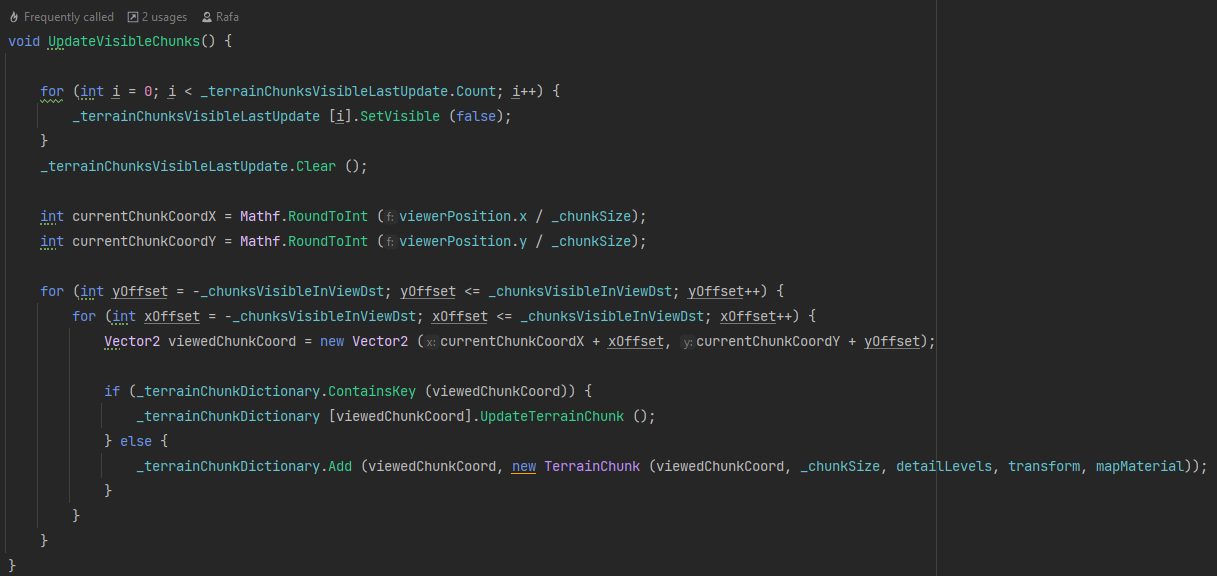
\includegraphics[width=1\textwidth]{img/codes/EndlessTerrain-updateVisibleChunks.png}
    \caption{Carga y descarga de chunks en función de la posición del jugador.}
\end{figure}

\subsubsection{Implementación de Niveles de Detalle (LOD)}

\textbf{Inicialización de parámetros:}

\begin{itemize}
    \item \textbf{Incremento de simplificación de la mesh}: Esta variable controla cuántos vértices se saltan durante la generación de la malla. Si levelOfDetail es 0, no se aplica simplificación, y se establece en 1. Si levelOfDetail es mayor que 0, meshSimplificationIncrement se establece en levelOfDetail * 2, lo que significa que se omiten más vértices en la generación de la malla a medida que aumenta el nivel de detalle.
    \item \textbf{Vértices por línea}:Esta variable determina el número de vértices por línea en la malla. Se calcula dividiendo (size - 1) por meshSimplificationIncrement y sumando 1. Cuanto mayor sea el valor de meshSimplificationIncrement, menor será la cantidad de vértices por línea, lo que resultará en una malla menos detallada.
\end{itemize}
\begin{figure}[h]
    \centering
    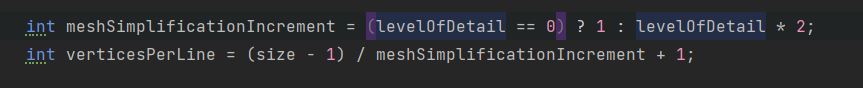
\includegraphics[width=1\textwidth]{img/codes/LOD-parametros.png}
    \caption{Inicialización de variables que implementan LOD.}
\end{figure}

\textbf{Aplicación de las variables de LOD:}

El bucle anidado que recorre el terreno usa meshSimplificationIncrement para determinar cuántos vértices procesar en cada iteración. Cuanto mayor sea meshSimplificationIncrement, menos iteraciones se realizarán en el bucle, lo que significa que se generará menos detalle en la malla. Los vértices omitidos no se incluirán en la malla final.

Triángulos en la malla: Los triángulos que forman la malla se crean en función de la posición de los vértices generados. Si meshSimplificationIncrement es mayor, se omitirán más vértices, lo que resultará en menos triángulos y, por lo tanto, en una malla más simplificada.

Aquí se muestra el código de la función:
\begin{figure}[h]
    \centering
    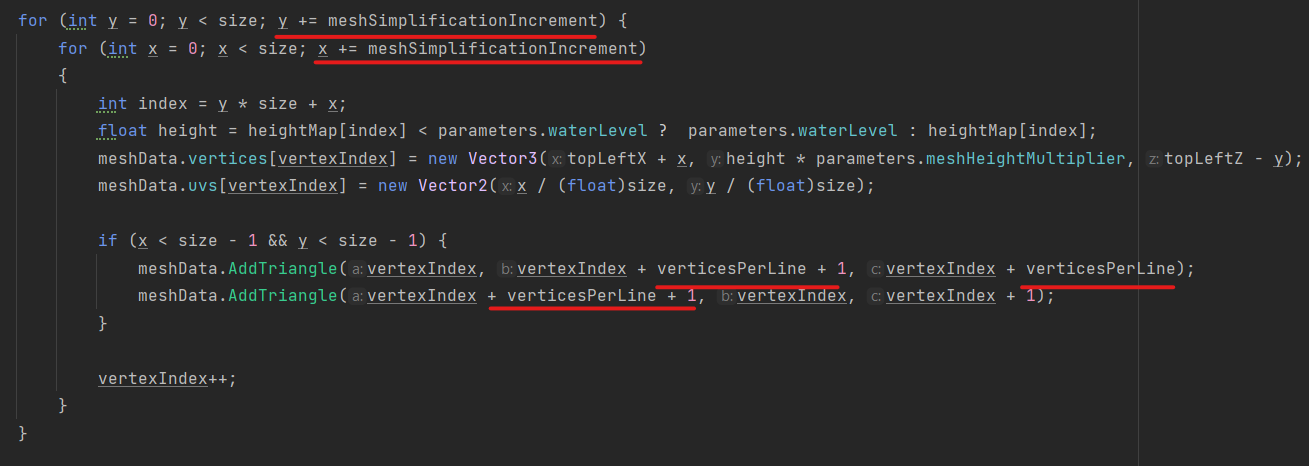
\includegraphics[width=1\textwidth]{img/codes/LOD-bucle.png}
    \caption{Bucle para construir la mesh con LOD.}
\end{figure}

\subsubsection{Generación de Valores de Ruido}

La generación de valores de ruido es un paso fundamental en la creación de terrenos realistas y variados. En este contexto, se utiliza el ruido para determinar las alturas y características del terreno generado. El algoritmo de generación de ruido se implementa en la clase \texttt{Noise} y puede utilizar diferentes tipos de ruido, como Perlin, Simplex o Voronoi, según los parámetros especificados.

\paragraph{Parámetros de Ruido}

Para generar el ruido, se utilizan varios parámetros que influyen en la apariencia del terreno:

\begin{itemize}
    \item \textbf{Tamaño del Mapa (\texttt{mapSize})}: El tamaño del mapa define cuántos puntos se generarán en el mapa de ruido. Cuanto mayor sea este valor, mayor será la resolución del terreno generado.
    
    \item \textbf{Configuración de Altura (\texttt{parameters})}: Esta configuración incluye información como la semilla (\texttt{seed}), la escala del ruido (\texttt{noiseScale}), la persistencia (\texttt{persistance}), la lacunaridad (\texttt{lacunarity}), el número de octavas (\texttt{octaves}) y el desplazamiento (\texttt{offset}). Estos parámetros ajustan cómo se combinarán y generarán los valores de ruido.
    
    \item \textbf{Tipo de Ruido (\texttt{noiseType})}: El algoritmo permite elegir entre diferentes tipos de ruido, como Perlin, Simplex o Voronoi. Cada tipo de ruido tiene un comportamiento único que afecta la apariencia del terreno.
\end{itemize}

\paragraph{Generación de Valores de Ruido}

El algoritmo de generación de ruido comienza con la inicialización de los parámetros, incluidos los desplazamientos aleatorios para cada octava. Luego, se procede a generar los valores de ruido para cada punto en el mapa.

\begin{enumerate}
    \item \textbf{Incialización de Parámetros}: Se generan desplazamientos aleatorios para cada octava, lo que permite variar el patrón de ruido en cada octava y controlar la aparición de detalles a diferentes escalas.
    Aquí se muestra el código:
    \begin{figure}[h]
        \centering
        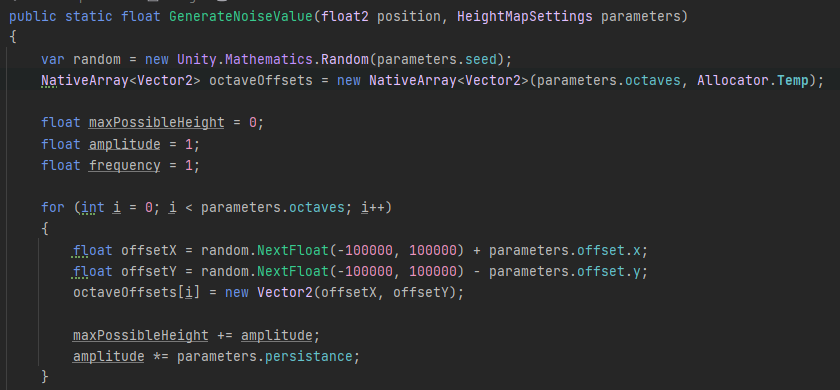
\includegraphics[width=0.9\textwidth]{img/codes/octavas.png}
        \caption{Generación de desplazamientos aleatorios para cada octava.}
    \end{figure}
    
    \item \textbf{Bucle de Generación}: Para cada punto en el mapa de tamaño \texttt{mapSize}, se calcula un valor de ruido. Esto se hace mediante la combinación de múltiples octavas de ruido, cada una escalada y ponderada adecuadamente. La suma de estos valores de ruido se utiliza como altura o característica del terreno en ese punto.
    \begin{figure}[h]
        \centering
        \includegraphics[width=0.9\textwidth]{img/codes/GeneraciónRuido.png}
        \caption{Generación de valores de ruido basado en parámeteros.}
    \end{figure}
    \item \textbf{Nótese cómo en el bucle de generación se multiplican los valores frecuencia y amplitud por la lacunaridad y la Persistencia respectivamente de manera que se aplican estos parámetrod en cada octava}
    \item \textbf{Normalización}: Los valores de ruido generados no están en el rango deseado. Se realiza una normalización para ajustar estos valores al rango [0, 1], que es más adecuado para representar alturas.
    \begin{figure}[h]
        \centering
        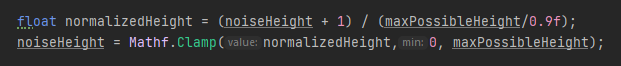
\includegraphics[width=0.9\textwidth]{img/codes/normalizacion.png}
        \caption{Normalización de los valores de ruido generados.}
    \end{figure}
\end{enumerate}

\paragraph{Tipo de Ruido}

El tipo de ruido utilizado afecta significativamente la apariencia del terreno:

\begin{itemize}
    \item \textbf{Perlin}: Este tipo de ruido proporciona un aspecto suave y ondulado al terreno. Es especialmente útil para crear formaciones de terreno natural, como colinas y montañas.
    
    \item \textbf{Simplex}: El ruido Simplex es conocido por su capacidad para generar terrenos más naturales y sin patrones visibles. Puede ser útil para terrenos detallados y variados.
    
    \item \textbf{Voronoi}: El ruido Voronoi se utiliza para crear patrones celulares y características geométricas en el terreno. Puede generar formaciones de terreno únicas y distintivas.
\end{itemize}

\begin{figure}[h]
    \centering
    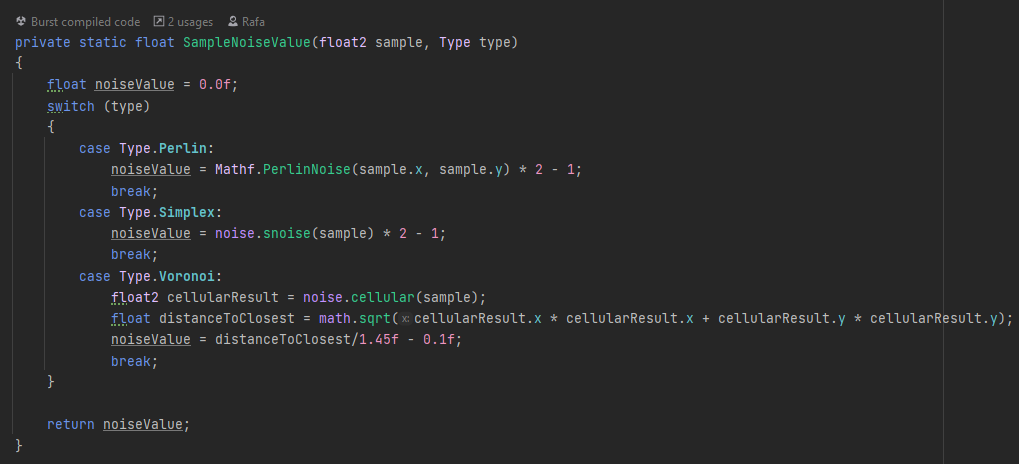
\includegraphics[width=1\textwidth]{img/codes/TiposRuido.png}
    \caption{Función para genrar un valor de ruido u otro en base al tipo seleccionado.}
\end{figure}

\subsubsection{Generación del Mapa de Altura}

\textbf{Llamada al Job desde clase Monobehaviour:}

La generación del mapa de altura se realiza mediante la ejecución de un job de Unity llamado MapDataGeneratorJob. Este job se encarga de calcular las alturas en función de las configuraciones proporcionadas y genera el mapa de altura correspondiente. La ejecución del job se realiza en paralelo, lo que aprovecha el rendimiento de sistemas multi-núcleo.

El Job es llamado desde un método en la clase Monobehaviour que hacede interfaz entre el Job y EndlessTerrain. En la siguiente imagen se observa el código donde se genera el gradiente de color y se hace la llamada al Job:
\begin{figure}[h]
    \centering
    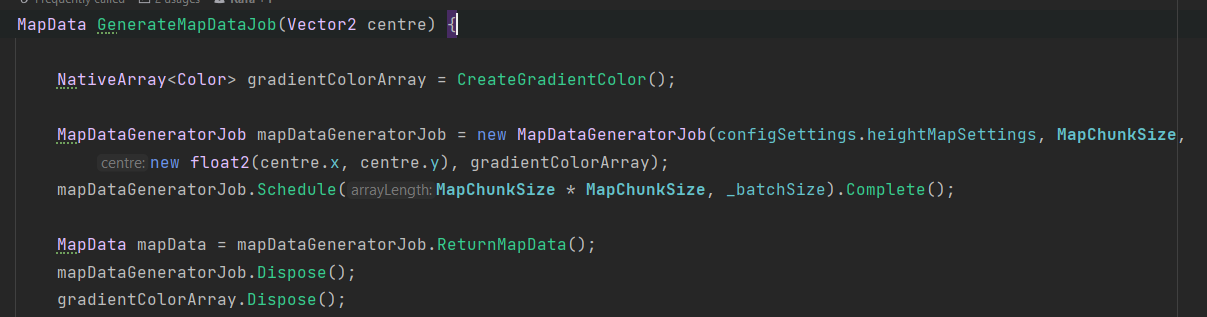
\includegraphics[width=0.9\textwidth]{img/codes/MapGenerator-GenerateMapData.png}
    \caption{Implementación del job MapDataGeneratorJob para la generación del mapa de altura.}
    \end{figure}

\textbf{Job:}

\begin{itemize}
\item \textbf{Cálculo de Alturas}: En cada iteración del job, se calcula la altura del terreno en una posición específica. Esto se logra utilizando funciones de ruido y las configuraciones de altura del terreno.
\item \textbf{Asignación de Colores}: Para cada punto en el mapa de altura, se asigna un color correspondiente utilizando la paleta de colores. Esta asignación se basa en la altura calculada previamente.

Aquí se muestra el código del método execute del MapDataGeneratorJob donde se obtiene la altura y el color para un vértice:
\begin{figure}[h]
    \centering
    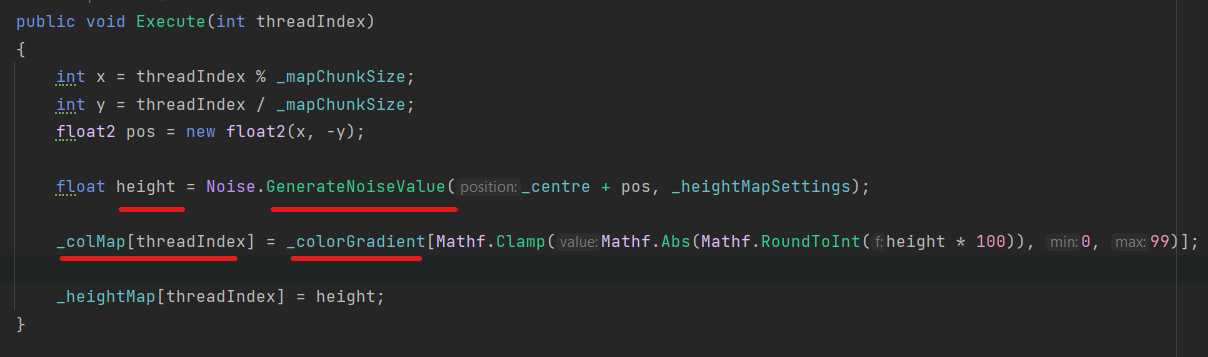
\includegraphics[width=0.9\textwidth]{img/codes/GenracionAlturaYColores.png}
    \caption{Generación de altura y color para un vértice.}
\end{figure}

\item \textbf{MapData Resultante}: El resultado de la generación del mapa de altura se encapsula en una estructura MapData, que contiene tanto el mapa de altura como el mapa de color.
\end{itemize}
\begin{figure}[h]
    \centering
    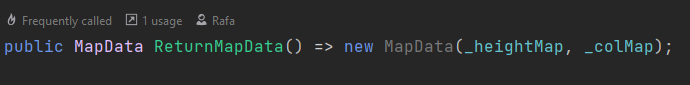
\includegraphics[width=0.9\textwidth]{img/codes/MapDataReturn.png}
    \caption{Generación de la estructura MapData con los datos.}
\end{figure}

Con la finalización de este proceso, se obtiene un mapa de altura que sirve como base para la generación del terreno y contribuye significativamente a su aspecto y forma finales.

Este mapa de altura se utiliza posteriormente en la creación de las mallas del terreno y en otros procesos relacionados con la generación procedural.

\subsubsection{Generación de las Mallas del Terreno}

\textbf{Llamada al Job desde Clase MonoBehaviour:}

La generación de la malla del terreno se lleva a cabo mediante la ejecución de un job de Unity llamado MeshDataGeneratorJob. Este job se encarga de calcular los vértices, triángulos y coordenadas UV de la malla en función de los datos del mapa de altura proporcionados. La ejecución del job se realiza en paralelo, lo que optimiza el rendimiento de la generación de mallas para terrenos de gran escala.

La llamada al job se efectúa desde un método en la clase MonoBehaviour que actúa como intermediario entre el job y el componente EndlessTerrain. En la siguiente imagen se muestra el código donde se crea un job de generación de malla y se ejecuta:

\begin{figure}[h]
\centering
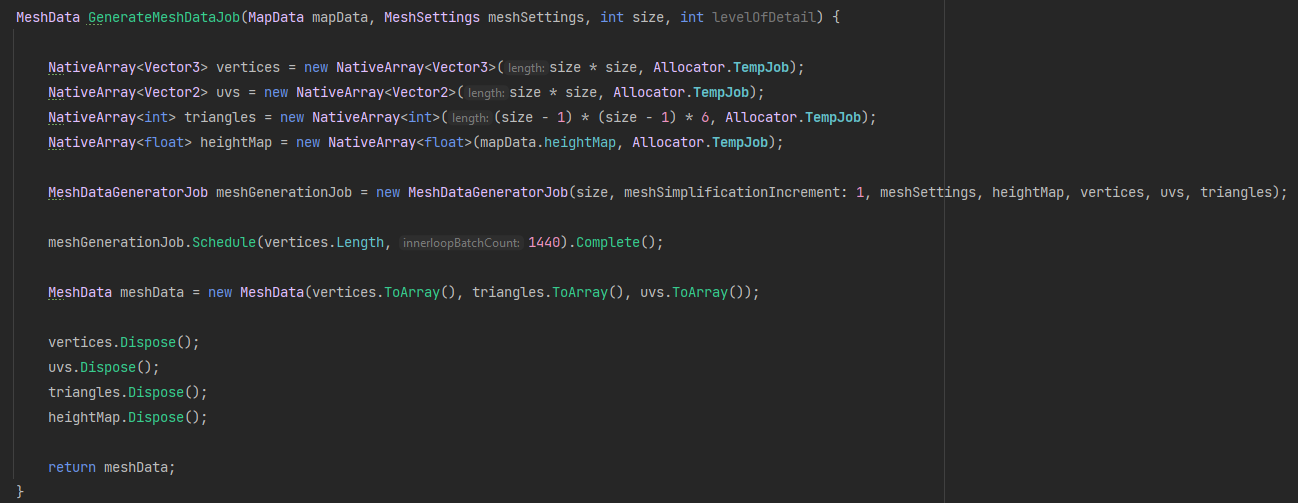
\includegraphics[width=1\textwidth]{img/codes/GenerateMeshData.png}
\caption{Implementación del job MeshDataGeneratorJob para la generación de la malla del terreno.}
\end{figure}

\textbf{Job:}

El job MeshDataGeneratorJob es responsable de generar los datos necesarios para crear la malla del terreno. A continuación, se describen los pasos clave de este proceso:

\begin{itemize}
\item \textbf{Cálculo de Vértices y Coordenadas UV}: En cada iteración del job, se calcula la posición de un vértice en la malla. La altura del vértice se obtiene a partir de los datos del mapa de altura, y las coordenadas UV se asignan en función de la posición en el terreno. Esto permite mapear texturas sobre la malla de manera adecuada. 

\begin{figure}[h]
    \centering
    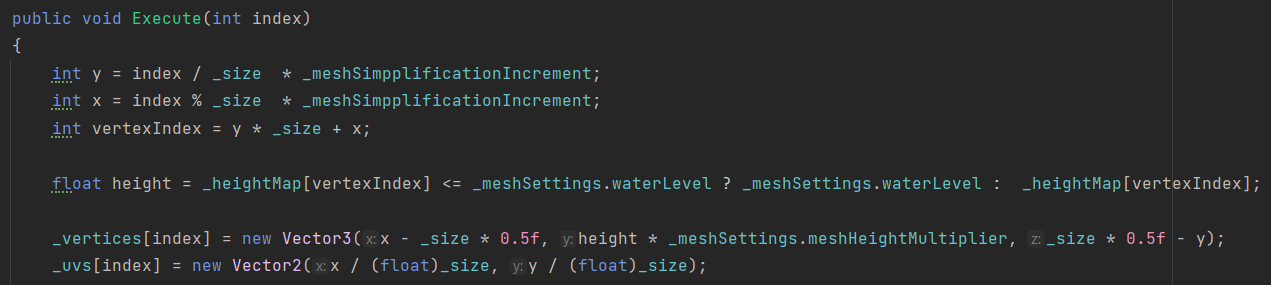
\includegraphics[width=1\textwidth]{img/codes/CalculoVerticesYUVs.png}
    \caption{Cálculo de los vértices y uvs en método Execute del Job.}
\end{figure}

\item \textbf{Creación de Triángulos}: Los triángulos que forman la malla se definen en función de los vértices calculados. Los triángulos determinan la conectividad de la malla y son esenciales para su representación gráfica.
\begin{figure}[h]
    \centering
    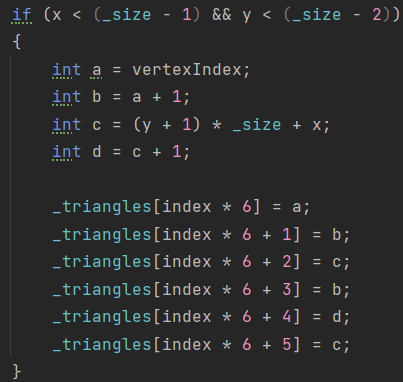
\includegraphics[width=0.5\textwidth]{img/codes/CalculoTriangulos.png}
    \caption{Cálculo de los triángulos en método Execute del Job.}
\end{figure} 
\item \textbf{Resultados en una Estructura}: Los datos generados, incluyendo los vértices, triángulos y coordenadas UV, se encapsulan en una estructura MeshData. Esta estructura almacena todos los elementos necesarios para construir la malla del terreno.
\begin{figure}[h]
    \centering
    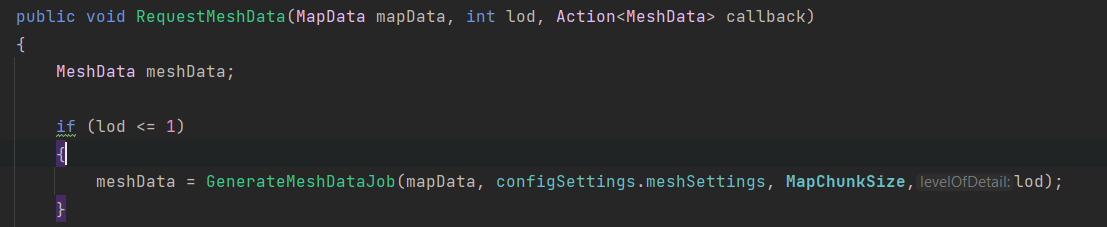
\includegraphics[width=1\textwidth]{img/codes/CreacionMeshData.png}
    \caption{Encapsulación de la información de la mesh en estructura MeshData.}
\end{figure}  
\end{itemize}

Con la finalización de este proceso, se obtiene una malla detallada que representa el terreno procedimental. El uso de jobs en paralelo permite una generación eficiente de la malla, lo que es fundamental para la representación de terrenos complejos y de gran escala en tiempo real.

\subsubsection{Aplicación de Algoritmos de Erosión}

\textbf{Llamada a la Erosión desde Clase MonoBehaviour:}

La aplicación de algoritmos de erosión en el terreno se logra mediante la función ApplyErosion, que utiliza un job de Unity llamado ErosionJob. La erosión es un proceso iterativo que simula la degradación del terreno con el tiempo. La función aplica erosión al mapa de alturas del terreno en múltiples ciclos, donde cada ciclo representa una iteración de erosión. El número de ciclos y otros parámetros de erosión se toman de la configuración.

En el siguiente código, se muestra cómo se llama a la función ApplyErosion y se ejecutan los ciclos de erosión:

\begin{figure}[h]
    \centering
    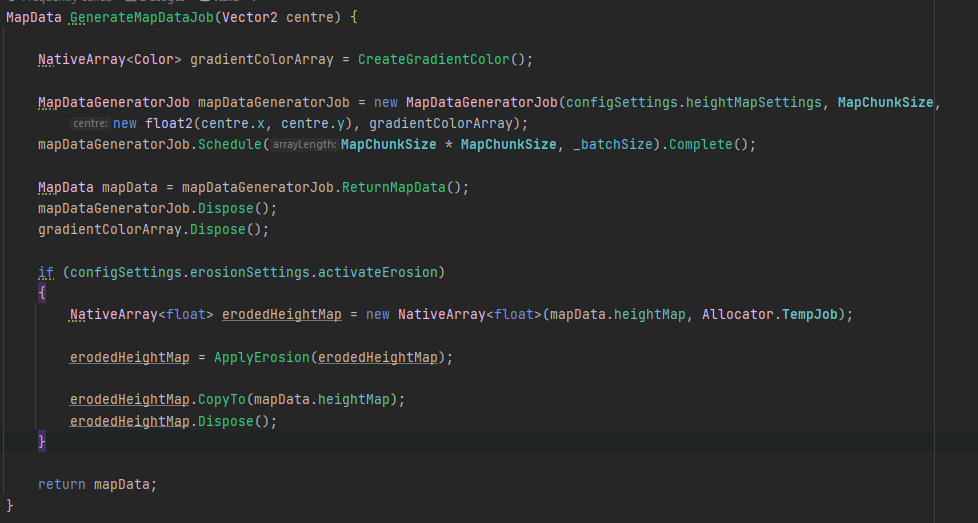
\includegraphics[width=1\textwidth]{img/codes/ApplyErosionCall.png}
    \caption{Llamada a ApplyErosion.}
\end{figure}  

\begin{figure}[h]
    \centering
    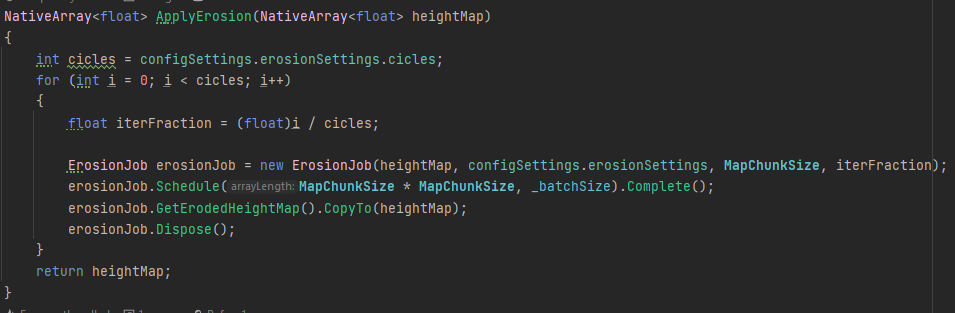
\includegraphics[width=1\textwidth]{img/codes/ApplyErosionFunction.png}
    \caption{Aplicación de la erosión.}
\end{figure} 

\textbf{Job de Erosión (ErosionJob):}

El job ErosionJob es responsable de aplicar la erosión al mapa de alturas. Aquí se describen los pasos clave realizados por el job:

\begin{itemize}
\item \textbf{Cálculo de la Altura Erosionada}: En cada iteración del job, se calcula la altura erosionada para cada punto en el mapa de alturas. Esto se hace evaluando las alturas de los vecinos y aplicando reglas específicas basadas en el ángulo de talud. La erosión reduce la altura del terreno en función de su pendiente y otros parámetros de erosión.
\item \textbf{Consideración de los Bordes}: Se tiene en cuenta si el punto está dentro del área del borde, y en función de esto, se aplica o no la erosión en el borde del mapa. Se pueden aplicar reglas de erosión diferentes en el borde y en el interior.
\item \textbf{Iteraciones de Erosión}: El job de erosión se ejecuta múltiples veces según el número de ciclos especificados en la configuración. En cada iteración, se aplica la erosión a los datos del mapa de alturas, y se disminuye la altura del terreno.
\end{itemize}

\begin{figure}[h]
\centering
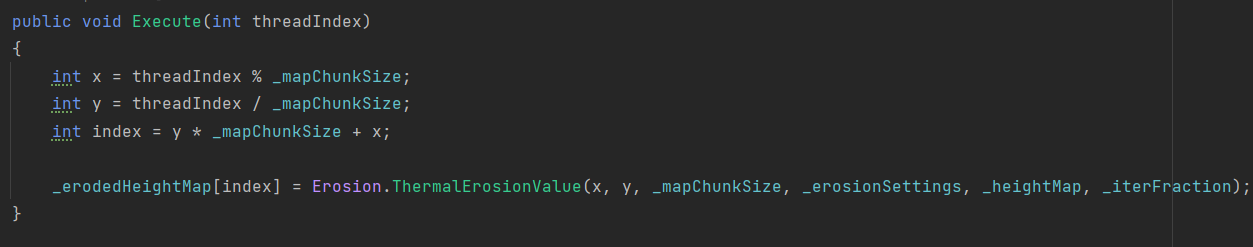
\includegraphics[width=1\textwidth]{img/codes/ExecuteErosionJob.png}
\caption{Implementación del método Execute de ErosionJob.}
\end{figure}

La erosión es un componente esencial para simular procesos realistas de degradación del terreno, como el suavizado de pendientes y la reducción de la aspereza. Su aplicación repetida a lo largo de varios ciclos permite modelar la evolución del terreno con el tiempo.
\subsubsection{Generación de Texturas del Terreno}

La generación de texturas del terreno se encarga de convertir el mapa de colores (colorMap) obtenido durante la generación de alturas en una textura adecuada para su visualización en el terreno. Esto se logra utilizando la clase \texttt{TextureGenerator}.

\subsubsection{Generación de texturas}

\begin{enumerate}
    \item \texttt{TextureFromColourMap}: Este método toma un arreglo de colores (\texttt{colourMap}), junto con el ancho y alto deseados, y crea una textura 2D a partir de estos datos. Configura la textura con un modo de filtrado (\texttt{Point}) y un modo de envoltura de textura que normaliza los valores. Luego, asigna los colores del \texttt{colourMap} y aplica la textura.

    \begin{figure}[h]
    \centering
    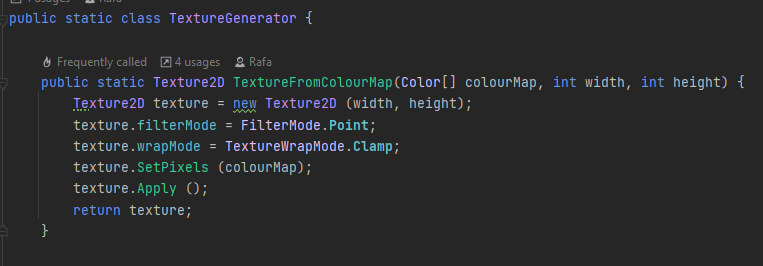
\includegraphics[width=0.85\textwidth]{img/codes/TextureColor.png}
    \caption{Implementación del método de generación de texturas.}
    \end{figure}
    \newpage
    \item \texttt{Uso en la Clase TerrainChunk}:En la clase \texttt{TerrainChunk}, específicamente en el método \texttt{OnMapDataReceived}, se utiliza la clase \texttt{TextureGenerator} para crear una textura a partir del mapa de colores (\texttt{colourMap}) contenido en el objeto \texttt{MapData} recibido. Luego, esta textura se asigna al material del terreno para su visualización en el objeto \texttt{\_meshRenderer}. A continuación se muestra el fragmento relevante de código:
    \begin{figure}[h]
        \centering
        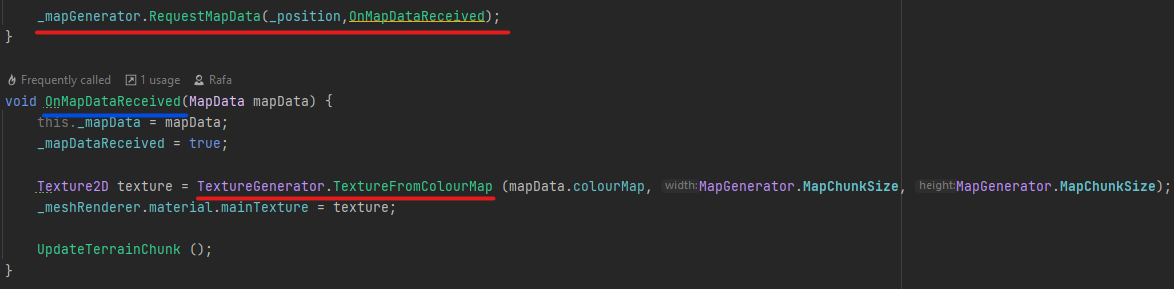
\includegraphics[width=0.85\textwidth]{img/codes/TexturizacionDeChunk.png}
        \caption{generación de textura al crearse un nuevo chunk.}
    \end{figure}
    
\end{enumerate}

\subsection{Elección de Estructuras de Datos y Tipos}

En esta sección se explicará por qué se han utilizado las estructuras de datos empleadas para la implementación de los trabajos y qué sentido tienen, dado que la elección de las estructuras viene en buena parte marcada por necesidades de implementación y optimización del rendimiento.

\subsubsection{Uso de structs en Jobs:}
El sistema de trabajos de Unity requiere que los trabajos sean tipos "no administrados", por lo que no pueden contener referencias a objetos. Las clases en C\# pueden contener referencias a otros objetos, lo que las hace más complejas y difíciles de optimizar. Esto se debe a que Job System está diseñado para funcionar con Burst Compiler, un compilador que optimiza el código generando código de máquina altamente optimizado que puede ejecutarse más rápido que el código C\# normal. Burst Compiler funciona mejor con tipos de datos simples que se pueden optimizar fácilmente, como las structs, por lo tanto, el uso de clases en el Job System de Unity puede provocar problemas de rendimiento, y es por esto que es preferible usar structs en lugar de clases, razón por la cual se han utilizado para el proyecto.

\subsubsection{NativeArrays:} 
El uso de NativeArrays en lugar de arrays de C\# se debe a que Burst Compiler está preparado para trabajar con estructuras de datos que permiten una optimización del código al pasarlo a lenguaje máquina. Los NativeArrays, a diferencia de los arrays normales, tienen una gestión de memoria eficiente, con posiciones contiguas donde almacenar los datos, de manera que no se produce fragmentación como sí podría ocurrir en los arrays de C\#. También almacenan los datos en zonas diferentes de la memoria que facilitan el acceso de manera más rápida y contribuyen a la eficiencia. Además, están preparados para que haya un acceso concurrente seguro de varios hilos a los datos que almacenan, por lo que permiten un manejo transparente al desarrollador de la concurrencia.

\subsubsection{Elección del tipo de Job:}
El tipo de job que se ha utilizado para el procesamiento de los vértices es IJobParallelFor, el cual divide el procesamiento de un número de posiciones de un array que se le pasa como parámetro en el método Schedule entre varios hilos, de manera óptima al ser un tipo de dato predefinido para ello. Dado que el tratamiento de los mapas de alturas y la creación de la malla es iterativo en su versión secuencial, el tener que paralelizar los bucles es una tarea que se realiza de manera óptima al usar un IJobParallelFor.


% Esta parte del código toma los datos de color del terreno, los convierte en una textura y luego asigna esa textura al material del terreno, lo que permite visualizar el terreno de manera adecuada en la escena de Unity.

% \subsection{Resolución de Problemas}

% En esta subsección, se abordan los problemas encontrados durante el desarrollo del sistema y se describe cómo se resolvieron. Se incluyen soluciones a desafíos específicos relacionados con la generación de terreno procedural en Unity.

% \begin{enumerate}
%     \item \textbf{Continuidad entre los chunks:}
%     \item \textbf{Separación entre los chunks:}
%     \item \textbf{Depresión de las zonas con agua:}
%     \item \textbf{Problemas de optimización temporal:}
%     \item \textbf{Problemas de optimización de memoria:}
%     \item \textbf{Problemas con continuidad de bordes al erosionar:}
%     \item \textbf{Problemas con rendimiento al erosionar:}
%     \item \textbf{Problemas con parametrización coherente:}
% \end{enumerate}
\chapter{Conclusiones}
% Contenidos del capítulo.
% Las secciones presentadas son orientativas y no representan
% necesariamente la organización que debe tener este capítulo.

\section{Conclusiones}

Este trabajo proporciona a cualquier interesado la capacidad de generar un terreno infinito y dinámico, de aspecto realista, mientras se desplaza por él. Gracias a los diversos tipos de ruido y configuraciones ajustables, esta herramienta ofrece una amplia variedad de combinaciones que permiten crear entornos personalizados con un buen rendimiento.

Esta herramienta es un recurso valioso y versátil, capaz de optimizar tanto el tiempo como los recursos necesarios para generar espacios de juego explorables. Al ser versatil y adaptable, esta herramienta se convierte en una sólida base para proyectos que requieran un terreno de juego personalizado e ilimitado.

\section{Trabajo futuro}
Como futuras líneas de trabajo se propone:

\begin{enumerate}
    \item \textbf{Mejora de la Interacción del Usuario:} Desarrollar una interfaz de usuario más amigable que permita a los creadores de contenido ajustar los parámetros y ver los cambios en tiempo real, lo que facilitaría la creación de terrenos a medida.
    
    \item \textbf{Optimización del Rendimiento:} Continuar trabajando en la optimización del rendimiento para garantizar que la generación de terrenos sea lo más eficiente posible, especialmente en entornos de tiempo real.
    
    \item \textbf{Más Algoritmos de Generación:} Investigar y agregar otros algoritmos de generación de terrenos, lo que brindaría a los usuarios aún más opciones y flexibilidad en la creación de entornos.
    
    \item \textbf{Integración de Simulación Climática:} Incorporar sistemas de simulación climática y de agua que permitan la creación de terrenos que respondan de manera realista a cambios climáticos y eventos naturales.
    
    \item \textbf{Generación Procedural de Biomas:} Expandir la generación procedural para incluir la creación automática de vegetación, animales y criaturas para poblaciones de entornos.
    
    \item \textbf{Herramientas de Escultura 3D:} Agregar herramientas de escultura 3D que permitan a los usuarios modelar y personalizar terrenos con mayor detalle.
    
    \item \textbf{Compatibilidad con Plataformas Externas:} Adaptable a otras plataformas o motores de juegos populares además de Unity para aumentar la accesibilidad de la herramienta.
    
    \item \textbf{Colaboración en Tiempo Real:} Facilitar la colaboración en tiempo real, lo que permitiría a varios usuarios trabajar juntos en la creación y edición de terrenos de manera simultánea.
    
    \item \textbf{Generación de Ciudades y Entornos Urbanos:} Ampliar la capacidad de la herramienta para generar ciudades y entornos urbanos completos, lo que sería útil para juegos de mundo abierto y simuladores urbanos.
    
    \item \textbf{Integración de Inteligencia Artificial:} Implementar algoritmos de IA que permitan que los terrenos se adapten y evolucionen de manera dinámica en función de las acciones de los jugadores o las condiciones del juego.
    
    \item \textbf{Compatibilidad con Realidad Virtual (RV) y Realidad Aumentada (RA):} Adaptable para su uso en entornos de RV y RA, lo que brindaría experiencias de juego más inmersivas y realistas.
    
    \item \textbf{Documentación y Comunidad:} Continuar mejorando la documentación y fomentar una comunidad activa de usuarios que compartan sus experiencias y desarrollos utilizando la herramienta.
\end{enumerate}






\pagestyle{appendix}

\appendix
\chapter{Apéndice}
\section{Cronograma de fases del desarrollo}

En el siguiente diagrama de Gantt se detalla el diseño de la duración de las tareas.

\begin{figure}[H]
    \centering
    \includegraphics[width=1\textwidth]{img/planificación gantt.png}
    \caption{Diagrama de Secuencia de Generación de Terreno.}
\end{figure}


\addcontentsline{toc}{chapter}{Bibliografía}
\bibliographystyle{unsrt}
\bibliography{bib/bibliografia}




\end{document}

%%% Local Variables:
%%% mode: latex
%%% TeX-master: t
%%% End:
